\documentclass[11pt,a4paper]{article}

\usepackage[margin=0.95in]{geometry}
\usepackage{amsmath,amssymb,amsfonts}
\usepackage{booktabs,array,tabularx,longtable,multirow,makecell}
\usepackage{graphicx,xcolor,float,caption,subcaption}
\usepackage{enumitem,microtype,setspace,parskip}
\usepackage{fancyhdr,titlesec}
\usepackage{listings}
\usepackage{cancel}
\usepackage{tcolorbox}
\tcbuselibrary{skins,breakable}
\usepackage{siunitx}
\usepackage{xurl}
\usepackage{tikz}
\usetikzlibrary{shapes.geometric,arrows.meta,positioning,calc,fit,backgrounds,decorations.pathreplacing}
\usepackage{pgfplots}
\pgfplotsset{compat=1.18}
\usepackage[numbers,sort&compress]{natbib}
\usepackage{hyperref}
\usepackage[nameinlink,capitalize]{cleveref}

\sisetup{detect-all,round-mode=places,round-precision=4}

\definecolor{auditblue}{RGB}{28,54,104}
\definecolor{auditgreen}{RGB}{20,90,50}
\definecolor{discrepancyred}{RGB}{125,32,32}
\definecolor{limitationgray}{RGB}{90,90,100}
\definecolor{auditgray}{RGB}{245,246,248}
\definecolor{quantumblue}{RGB}{10,60,140}
\definecolor{classicalteal}{RGB}{20,100,100}
\definecolor{audityellow}{RGB}{150,120,20}

\hypersetup{
  colorlinks=true,
  linkcolor=auditblue,
  citecolor=auditgreen,
  urlcolor=quantumblue,
  pdftitle={Independent Implementation, Reproduction, and Technical Audit of Adaptive Quantum Kernel Selection for WDBC Classification},
  pdfauthor={Independent WDBC Audit}
}

\titleformat{\section}{\large\bfseries\sffamily\color{auditblue}}{\thesection}{0.8em}{}[\titlerule]
\titleformat{\subsection}{\normalsize\bfseries\sffamily\color{auditblue!80!black}}{\thesubsection}{0.8em}{}
\titleformat{\subsubsection}{\normalsize\itshape\sffamily}{\thesubsubsection}{0.8em}{}

\pagestyle{fancy}
\fancyhf{}
\fancyhead[L]{\small\sffamily\color{auditblue} Independent WDBC Audit of Daga et al.\ (2026)}
\fancyhead[R]{\small\sffamily\thepage}
\fancyfoot[C]{\small\sffamily\color{gray} Academic implementation, reproduction, and technical audit}
\renewcommand{\headrulewidth}{0.4pt}

\setstretch{1.12}
\setlength{\parskip}{0.35em}
\setlist[itemize]{leftmargin=1.4em,itemsep=0.15em}
\setlist[enumerate]{leftmargin=1.4em,itemsep=0.15em}

% Shared macros and TikZ styles
\newcommand{\papername}{Daga et al.\ (2026)}
\newcommand{\wdbc}{WDBC}
\newcommand{\statusv}{\textsc{Verified}}
\newcommand{\statuss}{\textsc{Supported under tested protocol}}
\newcommand{\statusd}{\textsc{Implementation discrepancy}}
\newcommand{\statusm}{\textsc{Methodological limitation}}
\newcommand{\statusstat}{\textsc{Statistical limitation}}
\newcommand{\statusr}{\textsc{Reproducibility issue}}
\newcommand{\statusp}{\textsc{Partially verified}}
\newcommand{\statusn}{\textsc{Not reproduced}}
\newcommand{\statusi}{\textsc{Inconclusive}}

\tikzset{
  auditnode/.style={
    rectangle, rounded corners=3pt, draw=auditblue, fill=auditgray,
    align=center, font=\sffamily\small, inner sep=5pt, minimum height=0.72cm
  },
  qnode/.style={
    rectangle, rounded corners=3pt, draw=quantumblue, fill=quantumblue!8,
    align=center, font=\sffamily\small, inner sep=5pt, minimum height=0.72cm
  },
  cnode/.style={
    rectangle, rounded corners=3pt, draw=classicalteal, fill=classicalteal!8,
    align=center, font=\sffamily\small, inner sep=5pt, minimum height=0.72cm
  },
  rnode/.style={
    rectangle, rounded corners=3pt, draw=auditgreen, fill=auditgreen!8,
    align=center, font=\sffamily\small, inner sep=5pt, minimum height=0.72cm
  },
  dnode/.style={
    rectangle, rounded corners=3pt, draw=discrepancyred, fill=discrepancyred!6,
    align=center, font=\sffamily\small, inner sep=5pt, minimum height=0.72cm
  },
  annode/.style={
    rectangle, rounded corners=3pt, draw=limitationgray, fill=limitationgray!10,
    align=center, font=\sffamily\small, inner sep=5pt, minimum height=0.72cm
  },
  fatarrow/.style={-{Stealth[length=2.2mm]}, thick, auditblue},
}

\newcommand{\gatebox}[1]{%
  \tikz[baseline=(g.base)]{\node[draw=auditblue, fill=white, inner sep=2pt, font=\scriptsize\sffamily, rounded corners=1pt] (g) {#1};}%
}


\begin{document}

\begin{titlepage}
\centering
\vspace*{1.1cm}
{\Huge\bfseries\sffamily\color{auditblue}
Independent Implementation, Reproduction,\\[3pt]
and Technical Audit of Adaptive Quantum\\[3pt]
Kernel Selection for WDBC Classification}
\par\vspace{0.35cm}
{\Large\sffamily A Comparative Study with Daga et al.\ (2026)}
\par\vspace{0.45cm}
\rule{\textwidth}{1.4pt}
\par\vspace{0.25cm}
{\large\sffamily
Daga, Naole, Parikh, Bommineni \& Ramu,\\
``Adaptive quantum kernel selection via leakage-free stacking\\
for clinical diagnostics on NISQ hardware,''\\
\textit{Scientific Reports} \textbf{16}, 26840 (2026).\\
DOI: \texttt{10.1038/s41598-026-56928-1}
}
\par\vspace{0.2cm}
\rule{\textwidth}{0.8pt}
\par\vspace{0.55cm}

\begin{minipage}{0.92\textwidth}
\centering
\begin{tabular}{@{}ll@{}}
\toprule
\textbf{Empirical scope} & Wisconsin Diagnostic Breast Cancer (\wdbc) only \\
\textbf{Official repository} & \url{https://github.com/researchbackup27-sudo/Adaptive-Quantum-Kernel-Selection} \\
\textbf{Verified commit} & \texttt{23c89d350e5135080a8f4f7f012c4e98d1ee3f82} (\texttt{23c89d3}) \\
\textbf{Branch / tag} & \texttt{reproduction-verified-23c89d3} / \texttt{reproduction-wdbc-v1} \\
\textbf{Local path} & \texttt{C:/Research/Adaptive-Quantum-Kernel-Selection} \\
\textbf{Document type} & Independent implementation, reproduction, and technical audit \\
\bottomrule
\end{tabular}
\end{minipage}

\vspace{0.7cm}
\begin{minipage}{0.88\textwidth}
\sffamily\small
\textbf{Statement of scope.} All empirical analyses in this report are restricted to \wdbc\ unless explicitly stated otherwise. Parkinson's disease and Pima Indians Diabetes results from \papername\ are not analysed numerically here.
\end{minipage}

\vfill
{\sffamily\small\color{gray}
This report is an independent academic comparison of paper claims, released source-code behaviour, independent reproduction, and audit-defined experiments.\\
It is not affiliated with, endorsed by, or co-authored by Daga et al.}
\end{titlepage}

\tableofcontents
\newpage

\begin{abstract}
\noindent\textbf{Motivation.}
Kernel methods remain a natural baseline for moderately sized, moderately high-dimensional clinical tabular data. Quantum kernels have been proposed as alternative similarity measures on near-term simulators and hardware. Independent reproduction is required because paper methodology and executable code can diverge, and because simulated NISQ claims depend on circuit topology, noise model, and statistical protocol.

\noindent\textbf{Paper contribution.}
\papername\ describe quantum-kernel QSVM and QKNN classifiers, a classical RBF baseline, hard voting, out-of-fold (OOF) logistic stacking, and additional calibration, explainability, noise, and variational components, evaluated on multiple medical datasets including \wdbc.

\noindent\textbf{Scope.}
This report audits \wdbc\ only ($N=569$, $D=30$; 212 malignant / class~0; 357 benign / class~1). Other datasets in the paper are mentioned only as context.

\noindent\textbf{Independent implementation and reproduction.}
Using the unmodified released sources at commit \texttt{23c89d3} and cached $569\times569$ Gram matrices, the nine non-VQC \wdbc\ table entries (classical RBF, six quantum base learners, hard voting, OOF stacking) were reproduced at prediction level under the verified 10-fold protocol. Angle and amplitude kernels agree with closed-form overlaps to machine precision on sampled pairs; the clean ZZ/IQP kernel uses all-to-all $K_8$ connectivity in the tested primary code.

\noindent\textbf{Audits.}
Audit-defined experiments examined fold-local versus global preprocessing, exhaustive 4-of-6 subset selection, Holm correction of a 32-test RBF-comparator family, bounded nested classical tuning, leakage-controlled calibration, nested XAI, feature-backtracking algebra, clean-versus-noisy circuit topology, density-matrix noise, and ten CV seeds.

\noindent\textbf{Major discrepancies (technical, not accusatory).}
The released stacking quartet is hardcoded. The master VQC cost path severs autodiff under the tested PennyLane CPU configuration. The released noisy Angle/ZZ circuits differ from the clean kernels. The published raw-feature backtracking formula is algebraically dominated by PCA structure after normalisation.

\noindent\textbf{Conclusion.}
Under the audited \wdbc\ protocols, the non-VQC benchmark is independently reproducible, classical RBF remains strong, and the audited quantum stacking ensemble does not demonstrate superiority over classical RBF. Calibration is metric-dependent. Noisy simulation is not hardware validation. Parkinson's and Pima results, repaired full-scale VQC benchmarking, and physical NISQ execution are outside the present evidence.
\end{abstract}

\vspace{0.4em}
\noindent\textbf{Keywords:}
quantum kernels; QSVM; QKNN; stacking; nested cross-validation; data leakage; Holm correction; calibration; explainable AI; NISQ simulation; reproducibility; Wisconsin Diagnostic Breast Cancer.

\section{Introduction}
\label{sec:intro}

Support vector machines with radial-basis kernels remain competitive on small-to-moderate biomedical tables because they control capacity through a regularised maximum-margin problem in a reproducing kernel Hilbert space~\cite{cortes1995support,boser1992training,scholkopf2002learning}. Quantum kernels replace the classical inner product with a fidelity estimated from a parameterised feature map~\cite{havlicek2019quantum,schuld2019quantum,schuld2021supervised}. Interest in such kernels is scientific rather than automatic: quantum feature maps can be classically hard in some regimes~\cite{havlicek2019quantum,huang2021power}, yet medical tabular data need not possess that structure.

The Wisconsin Diagnostic Breast Cancer (\wdbc) set is a public, fully labelled, $N=569$ benchmark derived from nuclear morphometric features of fine-needle aspirates~\cite{street1993nuclear,mangasarian1995breast}. It is useful as a computational benchmark, not as a surrogate for prospective clinical validation.

Reproducibility requires more than matching a table to three decimals~\cite{pineau2021improving,kapoor2023leakage}. Source-code behaviour should be examined independently of paper prose. Statistical methodology matters because 10-fold scores are dependent~\cite{dietterich1998approximate,nadeau2003inference} and because many pairwise tests inflate family-wise error~\cite{holm1979simple}. Simulated NISQ claims require circuit-level verification: a depolarising channel applied to a different topology is not the same experiment as noisy execution of the clean kernel.

This report therefore distinguishes six categories that are not interchangeable:
\begin{enumerate}[label=\textbf{\Alph*.}]
  \item paper claims of \papername;
  \item behaviour of the released source at commit \texttt{23c89d3};
  \item our independent reproduction of that executable pipeline;
  \item our independent audit of methodology and artefacts;
  \item audit-defined corrected experiments;
  \item optional future work.
\end{enumerate}

\paragraph{Research questions.}
\begin{description}[style=nextline,leftmargin=2.2em]
  \item[RQ1] How closely can the \wdbc\ results be independently reproduced?
  \item[RQ2] Are the paper's described circuits consistent with the released executable circuits?
  \item[RQ3] Does the released implementation actually implement adaptive subset/model selection?
  \item[RQ4] How do the quantum ensemble results compare with classical baselines under fair tuning?
  \item[RQ5] Are statistical conclusions robust to multiplicity, fold dependence, preprocessing protocol, and CV seed?
  \item[RQ6] Are calibration, XAI, and noise claims supported by the implementation?
\end{description}

\section{Research motivation}
\label{sec:motivation}

Three practical questions motivate an independent \wdbc\ study. First, quantum-kernel pipelines are expensive to recompute; cached Gram matrices must be checked against closed forms and against PSD/symmetry diagnostics. Second, ensemble and stacking claims can hide selection leakage~\cite{wolpert1992stacked,varma2006bias,cawley2010overfitting,kapoor2023leakage}. Third, clinical-sounding language (calibration, XAI, NISQ robustness) can outrun the executable protocol. The motivation is methodological: to map what matched, what differed, what we added, and what the evidence does not establish.

\section{Statement of scope and evidence categories}
\label{sec:scope}

\begin{center}
\fbox{\parbox{0.92\textwidth}{\sffamily\bfseries All empirical analyses in this report are restricted to \wdbc\ unless explicitly stated otherwise.}}
\end{center}

\Cref{fig:evidence-hierarchy} summarises why paper text, released code, reproduction, audit, and corrected experiments must not be conflated.

\begin{figure}[H]
\centering
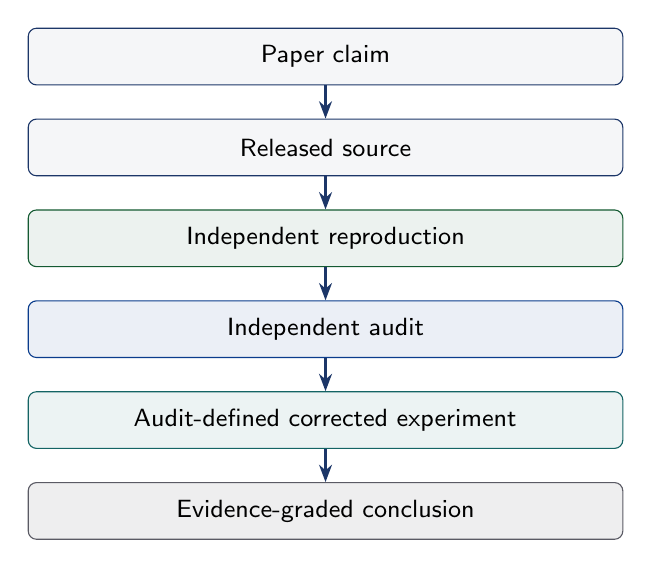
\begin{tikzpicture}[
  node distance=0.42cm,
  every node/.style={font=\sffamily\small}
]
\node[auditnode, text width=7.2cm] (p) {Paper claim};
\node[auditnode, text width=7.2cm, below=of p] (s) {Released source};
\node[rnode, text width=7.2cm, below=of s] (r) {Independent reproduction};
\node[qnode, text width=7.2cm, below=of r] (a) {Independent audit};
\node[cnode, text width=7.2cm, below=of a] (c) {Audit-defined corrected experiment};
\node[annode, text width=7.2cm, below=of c] (e) {Evidence-graded conclusion};
\draw[fatarrow] (p) -- (s);
\draw[fatarrow] (s) -- (r);
\draw[fatarrow] (r) -- (a);
\draw[fatarrow] (a) -- (c);
\draw[fatarrow] (c) -- (e);
\end{tikzpicture}
\caption{Evidence hierarchy used throughout this report. These layers are not interchangeable.}
\label{fig:evidence-hierarchy}
\end{figure}

\section{Literature review}
\label{sec:lit}

\subsection{Classical machine learning for \wdbc\ and small medical datasets}

\wdbc\ arose from computer-assisted cytometric analysis of breast FNA nuclei~\cite{street1993nuclear,wolberg1995breast,mangasarian1995breast}. With $N=569$ and $D=30$, linear and kernel methods, trees, and ensembles are all feasible. The majority-class rate is $357/569=0.6274$ (benign). High accuracy is therefore expected from strong classical models; incremental gains must be interpreted against that ceiling and against class encoding (here class~1 is benign).

\subsection{Support vector machines and RBF kernels}

The hard-margin SVM~\cite{boser1992training} and soft-margin formulation~\cite{cortes1995support} remain standard. Gaussian RBF kernels $K(x,z)=\exp(-\gamma\|x-z\|^2)$ induce a smooth similarity on $\mathbb{R}^d$~\cite{scholkopf2002learning}. In scikit-learn, \texttt{SVC(kernel='rbf', C=1, gamma='scale')} is a documented default configuration~\cite{pedregosa2011scikit}.

\subsection{Quantum kernel methods}

A quantum feature map $U(x)$ prepares $\lvert\phi(x)\rangle$; a kernel is typically the fidelity
\begin{equation}
K(x,z)=\lvert\langle\phi(x)\lvert\phi(z)\rangle\rvert^2,
\label{eq:fid}
\end{equation}
estimated by embedding $x$, uncomputing $z$, and reading the all-zero probability~\cite{havlicek2019quantum,schuld2019quantum}. Many supervised QML models are kernel methods in this sense~\cite{schuld2021supervised}. Advantage is data-dependent~\cite{huang2021power}.

\subsection{Quantum SVM and precomputed quantum-kernel classification}

Rebentrost et al.\ analysed a quantum algorithm for SVM in a different computational model~\cite{rebentrost2014quantum}. The pipeline audited here is the practical NISQ-era hybrid: precompute a Gram matrix on a simulator, then fit a classical SVM on that kernel~\cite{havlicek2019quantum,bergholm2018pennylane,pedregosa2011scikit}.

\subsection{Quantum $k$-NN and kernel-distance approaches}

Cover and Hart established nearest-neighbour classification~\cite{cover1967nearest}. Quantum distance classifiers can use interference to score similarity~\cite{schuld2017implementing}. In the released implementation, QKNN is a classical $k$-NN operating on distances derived from the quantum kernel matrix, not a hardware interference circuit.

\subsection{Ensemble learning and stacking}

Bagging~\cite{breiman1996bagging}, random forests~\cite{breiman2001random}, gradient-boosted trees~\cite{chen2016xgboost}, and stacked generalisation~\cite{wolpert1992stacked} combine base learners. Leakage-free stacking requires that meta-features for a sample not use that sample's training-fold labels~\cite{wolpert1992stacked,kapoor2023leakage}.

\subsection{Nested cross-validation and leakage-free preprocessing}

Fitting scalers or PCA on the full dataset before CV is a leakage pattern~\cite{kapoor2023leakage}. Nested CV reduces selection bias when models or subsets are chosen using inner scores~\cite{varma2006bias,cawley2010overfitting}. PCA itself is a linear variance decomposition~\cite{jolliffe2016pca}.

\subsection{Multiple hypothesis testing and Holm correction}

Holm's sequentially rejective procedure controls family-wise error more powerfully than Bonferroni~\cite{holm1979simple}. McNemar's test compares paired binary correctness~\cite{mcnemar1947note,dietterich1998approximate}; it is not a test of precision, recall, or specificity.

\subsection{Calibration of probabilistic classifiers}

Platt scaling maps SVM scores to probabilities~\cite{platt1999probabilistic}. Reliability diagrams, Brier score~\cite{brier1950verification}, and expected calibration error~\cite{naeini2015obtaining,niculescu2005predicting} quantify calibration. scikit-learn's \texttt{CalibratedClassifierCV} can calibrate \texttt{decision\_function} when available~\cite{pedregosa2011scikit}.

\subsection{Explainable AI and attribution stability}

SHAP provides additive feature attributions with game-theoretic axioms~\cite{lundberg2017unified}. LIME fits local surrogate models~\cite{ribeiro2016why}. Rank agreement among coefficient magnitude, SHAP, and permutation importance on linear meta-features is expected when the model is essentially linear in those features.

\subsection{NISQ noise simulation and circuit topology}

Preskill's NISQ framing emphasises limited fidelity and connectivity~\cite{preskill2018quantum}. Depolarising channels are phenomenological simulator knobs, not automatically measured hardware error rates. Topology (all-to-all versus a path graph) changes two-qubit gate count and the implemented kernel.

\subsection{Reproducibility and open-source research}

Open code is necessary but not sufficient~\cite{pineau2021improving}. PennyLane provides differentiable quantum circuits~\cite{bergholm2018pennylane}; autodiff can still be severed by Python-level collection of QNode outputs. Barren-plateau theory~\cite{mcclean2018barren} should not be inferred from a zero-gradient autodiff defect.

\section{Daga et al.\ (2026) methodology}
\label{sec:daga-methods}

As described in the paper, the clinical pipeline (category~A) comprises: (i)~standardisation, PCA to eight components, and scaling into a quantum-compatible interval; (ii)~multiple quantum feature maps; (iii)~QSVM and QKNN base learners plus classical comparators; (iv)~selection among base models; (v)~hard voting and OOF logistic stacking; (vi)~optional VQC, calibration, XAI, and noise studies; (vii)~evaluation on several datasets, of which only \wdbc\ is in our empirical scope.

\section{Released repository implementation}
\label{sec:released}

Category~B is the executable at commit \texttt{23c89d3}~\cite{daga2026repo}. Primary file \texttt{quantum\_clinical\_github.py} defines:
\begin{itemize}
  \item \texttt{qml.AngleEmbedding} on 8~wires (PennyLane default rotation axis $X$ in the tested configuration);
  \item \texttt{qml.IQPEmbedding} on 8~wires (all-to-all pattern in the clean kernel);
  \item \texttt{qml.AmplitudeEmbedding} on 3~wires with normalisation;
  \item QSVM/QKNN on precomputed kernels; classical RBF, RF, XGBoost, and classical stacking;
  \item hardcoded \texttt{BASE\_MODEL\_NAMES} at line~787;
  \item \texttt{qnn\_cost} collecting QNode outputs in a Python list;
  \item a separate noisy-circuit path using \texttt{default.mixed}.
\end{itemize}
\texttt{base\_model\_selection\_mcnemar.py} prints McNemar tables; it does not write a selected quartet back into the stacking script.

\section{Our independent implementation}
\label{sec:ours}

Category~C re-executes the released non-VQC \wdbc\ pipeline without modifying original research files. Category~D inspects circuits, statistics, and artefacts. Category~E adds fold-local preprocessing, nested 4-of-6 selection, Holm families, nested classical tuning, calibration/XAI/noise/seed audits, and a graph-preserving VQC gradient test. Cached Gram matrices in \texttt{checkpoints/} were used after independent structural and closed-form checks.

% diagrams.tex - Comprehensive TikZ Visualizations for the WDBC Audit
\section{System Architecture and Methodological Visualizations}
\label{sec:system-diagrams}

\subsection{End-to-End Hybrid Quantum-Classical Pipeline}
\Cref{fig:pipeline} illustrates the complete experimental architecture evaluated on the \wdbc\ benchmark ($N=569$, $D=30$). The pipeline integrates data preprocessing, quantum feature maps, Gram matrix generation, base classifier fitting, and out-of-fold logistic stacking alongside an independent classical comparison branch.

\begin{figure}[H]
\centering
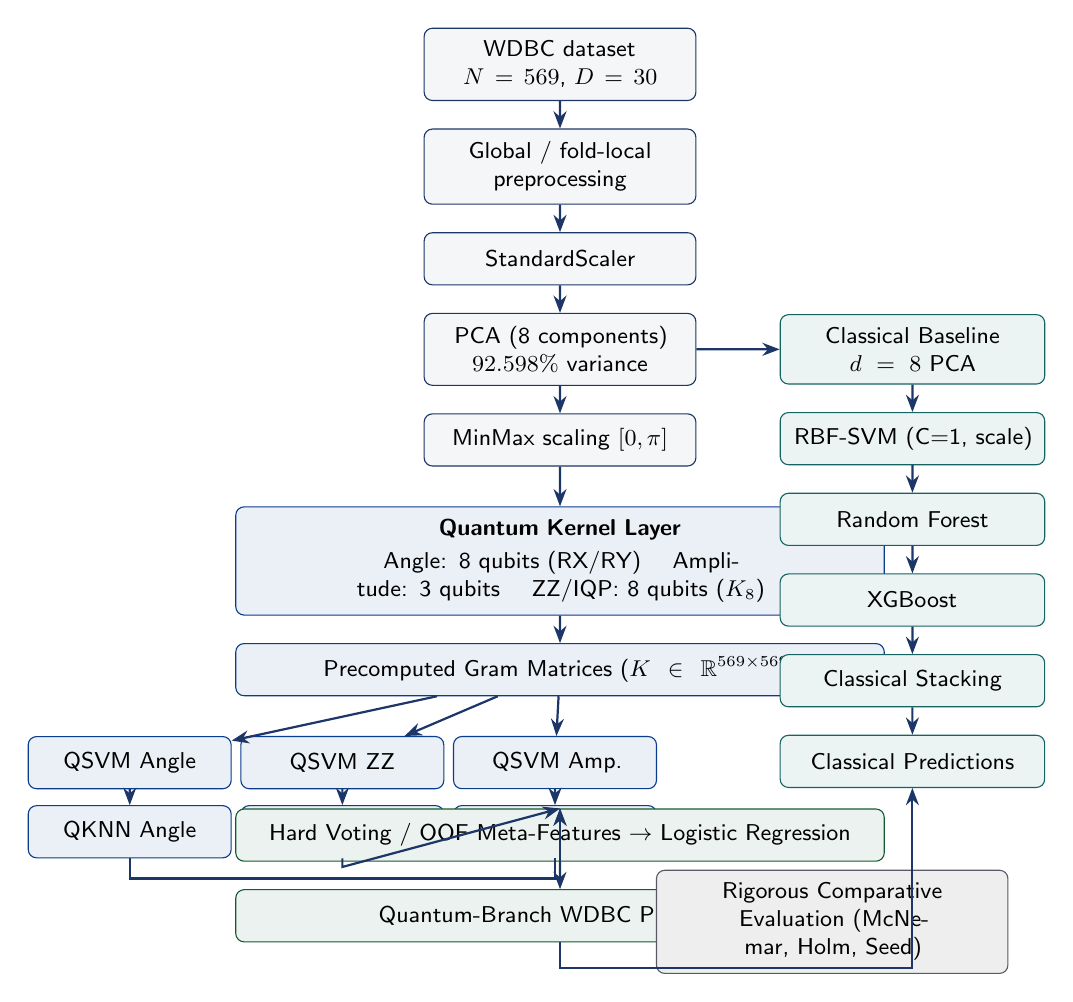
\begin{tikzpicture}[
  node distance=0.38cm and 0.45cm,
  every node/.style={font=\sffamily},
  scale=0.92, transform shape
]
\node[auditnode, text width=3.4cm] (data) {WDBC dataset\\$N=569$, $D=30$};
\node[auditnode, text width=3.4cm, below=of data] (pre) {Global / fold-local\\preprocessing};
\node[auditnode, text width=3.4cm, below=of pre] (ss) {StandardScaler};
\node[auditnode, text width=3.4cm, below=of ss] (pca) {PCA (8 components)\\$92.598\%$ variance};
\node[auditnode, text width=3.4cm, below=of pca] (mm) {MinMax scaling $[0,\pi]$};

\node[qnode, text width=8.6cm, below=0.55cm of mm] (qk) {%
\textbf{Quantum Kernel Layer}\\[2pt]
Angle: 8 qubits (RX/RY) \quad Amplitude: 3 qubits \quad ZZ/IQP: 8 qubits ($K_8$)};

\node[qnode, text width=8.6cm, below=of qk] (gram) {Precomputed Gram Matrices ($K \in \mathbb{R}^{569 \times 569}$)};

\node[qnode, text width=2.45cm, below left=0.55cm and 0.05cm of gram] (ba) {QSVM Angle};
\node[qnode, text width=2.45cm, right=0.12cm of ba] (bz) {QSVM ZZ};
\node[qnode, text width=2.45cm, right=0.12cm of bz] (bm) {QSVM Amp.};
\node[qnode, text width=2.45cm, below=0.22cm of ba] (ka) {QKNN Angle};
\node[qnode, text width=2.45cm, below=0.22cm of bz] (kz) {QKNN ZZ};
\node[qnode, text width=2.45cm, below=0.22cm of bm] (km) {QKNN Amp.};

\node[rnode, text width=8.6cm, below=1.55cm of gram] (ens) {Hard Voting / OOF Meta-Features $\to$ Logistic Regression};
\node[rnode, text width=8.6cm, below=of ens] (outq) {Quantum-Branch \wdbc\ Prediction};

\node[cnode, text width=3.3cm, right=1.15cm of pca] (cdata) {Classical Baseline\\$d=8$ PCA};
\node[cnode, text width=3.3cm, below=of cdata] (rbf) {RBF-SVM (C=1, scale)};
\node[cnode, text width=3.3cm, below=of rbf] (rf) {Random Forest};
\node[cnode, text width=3.3cm, below=of rf] (xgb) {XGBoost};
\node[cnode, text width=3.3cm, below=of xgb] (cst) {Classical Stacking};
\node[cnode, text width=3.3cm, below=of cst] (cout) {Classical Predictions};

\node[annode, text width=4.5cm] at ($(outq.east)!0.5!(cout.west)+(0,-1.15)$) {Rigorous Comparative\\Evaluation (McNemar, Holm, Seed)};

\foreach \a/\b in {data/pre,pre/ss,ss/pca,pca/mm,mm/qk,qk/gram,gram/ba,gram/bz,gram/bm,ba/ka,bz/kz,bm/km,ens/outq,cdata/rbf,rbf/rf,rf/xgb,xgb/cst,cst/cout}
  {\draw[fatarrow] (\a) -- (\b);}
\draw[fatarrow] (ka.south) -- ++(0,-0.28) -| (ens.north);
\draw[fatarrow] (kz.south) -- ++(0,-0.12) -- (ens.north);
\draw[fatarrow] (km.south) -- ++(0,-0.28) -| (ens.north);
\draw[fatarrow] (outq.south) -- ++(0,-0.35) -| (cout.south);
\draw[fatarrow] (pca.east) -- (cdata.west);
\end{tikzpicture}
\caption{System architecture of the audited \wdbc\ pipeline. Quantum and classical branches undergo paired 10-fold cross-validation on identical splits.}
\label{fig:pipeline}
\end{figure}

\subsection{Audit Methodology and Verification Hierarchy}
\Cref{fig:workflow} depicts the multi-tiered verification hierarchy applied throughout this investigation. Findings are partitioned into empirical reproduction, diagnostic audits, and audit-defined corrected experiments.

\begin{figure}[H]
\centering
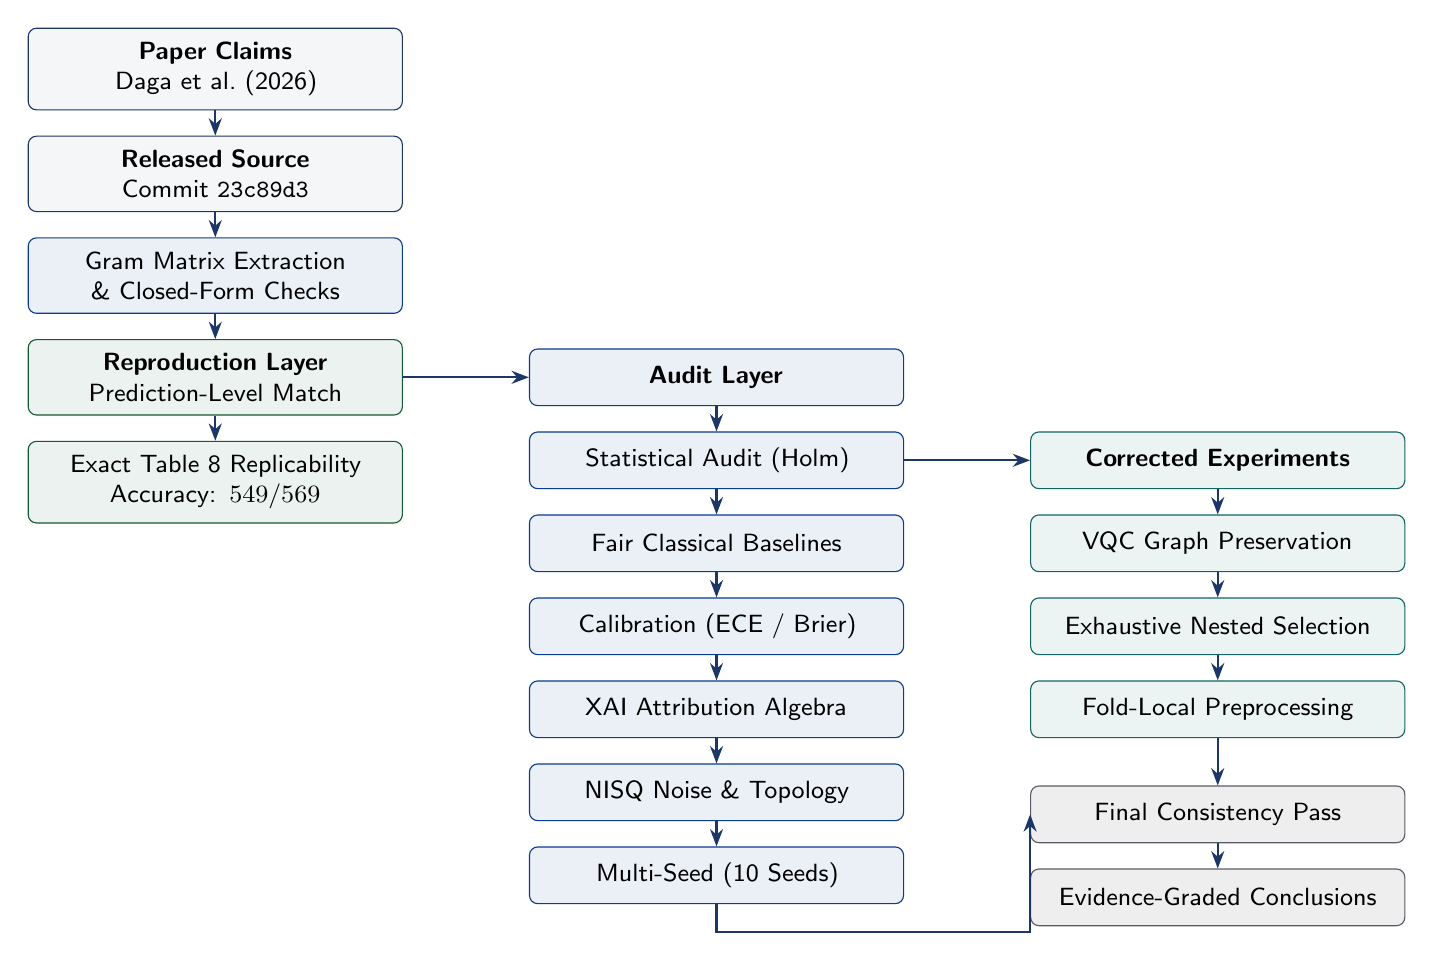
\begin{tikzpicture}[node distance=0.32cm, every node/.style={font=\sffamily\small}]
\node[auditnode, text width=4.4cm] (p) {\textbf{Paper Claims}\\Daga et al.\ (2026)};
\node[auditnode, text width=4.4cm, below=of p] (s) {\textbf{Released Source}\\Commit \texttt{23c89d3}};
\node[qnode, text width=4.4cm, below=of s] (e) {Gram Matrix Extraction\\\& Closed-Form Checks};
\node[rnode, text width=4.4cm, below=of e] (r) {\textbf{Reproduction Layer}\\Prediction-Level Match};
\node[rnode, text width=4.4cm, below=of r] (m) {Exact Table 8 Replicability\\Accuracy: $549/569$};

\node[qnode, text width=4.4cm, right=1.6cm of r] (a) {\textbf{Audit Layer}};
\node[qnode, text width=4.4cm, below=of a] (st) {Statistical Audit (Holm)};
\node[qnode, text width=4.4cm, below=of st] (f) {Fair Classical Baselines};
\node[qnode, text width=4.4cm, below=of f] (c) {Calibration (ECE / Brier)};
\node[qnode, text width=4.4cm, below=of c] (x) {XAI Attribution Algebra};
\node[qnode, text width=4.4cm, below=of x] (n) {NISQ Noise \& Topology};
\node[qnode, text width=4.4cm, below=of n] (sd) {Multi-Seed (10 Seeds)};

\node[cnode, text width=4.4cm, right=1.6cm of st] (corr) {\textbf{Corrected Experiments}};
\node[cnode, text width=4.4cm, below=of corr] (vqc) {VQC Graph Preservation};
\node[cnode, text width=4.4cm, below=of vqc] (nest) {Exhaustive Nested Selection};
\node[cnode, text width=4.4cm, below=of nest] (leak) {Fold-Local Preprocessing};
\node[annode, text width=4.4cm, below=0.6cm of leak] (qc) {Final Consistency Pass};
\node[annode, text width=4.4cm, below=of qc] (con) {Evidence-Graded Conclusions};

\foreach \a/\b in {p/s,s/e,e/r,r/m,a/st,st/f,f/c,c/x,x/n,n/sd,corr/vqc,vqc/nest,nest/leak,leak/qc,qc/con}
  {\draw[fatarrow] (\a) -- (\b);}
\draw[fatarrow] (r.east) -- (a.west);
\draw[fatarrow] (st.east) -- (corr.west);
\draw[fatarrow] (sd.south) -- ++(0,-0.35) -| (qc.west);
\end{tikzpicture}
\caption{Systematic audit workflow separating reproduction, diagnostic audits, and corrected experiments.}
\label{fig:workflow}
\end{figure}

\subsection{Quantum Circuit Topology Mismatch: Clean vs.\ Noisy ZZ Kernels}
\Cref{fig:circuit-topology} details the architectural disparity uncovered in the ZZ/IQP feature map. The clean baseline executes an all-to-all complete graph $K_8$ comprising 28 interaction pairs (56 CNOT gates). Conversely, the released NISQ simulation silently substitutes a 1D linear chain $P_8$ with only 7 interaction pairs (14 CNOT gates), representing a $75\%$ reduction in two-qubit entangling operations.

\begin{figure}[H]
\centering
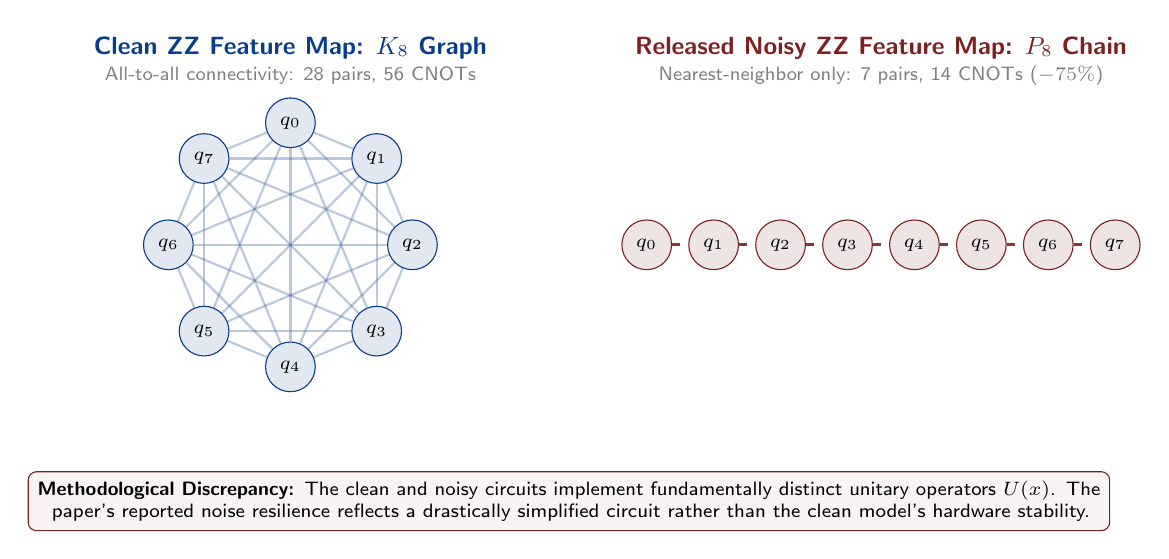
\begin{tikzpicture}[
  qubit/.style={circle, draw=quantumblue, fill=quantumblue!12, minimum size=0.55cm, font=\scriptsize\bfseries\sffamily},
  rqubit/.style={circle, draw=discrepancyred, fill=discrepancyred!12, minimum size=0.55cm, font=\scriptsize\bfseries\sffamily},
  edge_clean/.style={draw=quantumblue!80, thick},
  edge_noisy/.style={draw=discrepancyred!90, very thick, dashed}
]
% Left: Clean K_8
\node[font=\small\bfseries\sffamily\color{quantumblue}] at (0, 2.5) {Clean ZZ Feature Map: $K_8$ Graph};
\node[font=\scriptsize\sffamily\color{gray}] at (0, 2.15) {All-to-all connectivity: 28 pairs, 56 CNOTs};
\foreach \i in {0,1,...,7} {
  \node[qubit] (q\i) at ({90 - 45*\i}: 1.55cm) {$q_\i$};
}
\foreach \i in {0,1,...,6} {
  \foreach \j in {\the\numexpr\i+1\relax,...,7} {
    \draw[edge_clean, opacity=0.35] (q\i) -- (q\j);
  }
}

% Right: Noisy P_8
\begin{scope}[xshift=7.5cm]
\node[font=\small\bfseries\sffamily\color{discrepancyred}] at (0, 2.5) {Released Noisy ZZ Feature Map: $P_8$ Chain};
\node[font=\scriptsize\sffamily\color{gray}] at (0, 2.15) {Nearest-neighbor only: 7 pairs, 14 CNOTs ($-75\%$)};
\foreach \i in {0,1,...,7} {
  \node[rqubit] (p\i) at ({(\i - 3.5)*0.85cm}, 0) {$q_\i$};
}
\foreach \i in {0,1,...,6} {
  \pgfmathtruncatemacro{\next}{\i+1}
  \draw[edge_noisy] (p\i) -- (p\next);
}
\end{scope}

\node[draw=discrepancyred, fill=discrepancyred!5, rounded corners=3pt, text width=13.5cm, align=center, font=\scriptsize\sffamily, below=2.1cm of $(q4)!0.5!(p3)$] {
  \textbf{Methodological Discrepancy:} The clean and noisy circuits implement fundamentally distinct unitary operators $U(x)$. The paper's reported noise resilience reflects a drastically simplified circuit rather than the clean model's hardware stability.
};
\end{tikzpicture}
\caption{Architectural comparison between clean ($K_8$) and released noisy ($P_8$) ZZ feature maps.}
\label{fig:circuit-topology}
\end{figure}

\subsection{VQC Autograd Severance Mechanism}
\Cref{fig:vqc-severance} traces the exact point of autodiff failure in the author's VQC script (\texttt{vqc\_ablation\_and\_calibration\_github.py}). Python list comprehension strips tensor tracking, collapsing the backpropagation graph and forcing the parameter gradient norm to zero.

\begin{figure}[H]
\centering
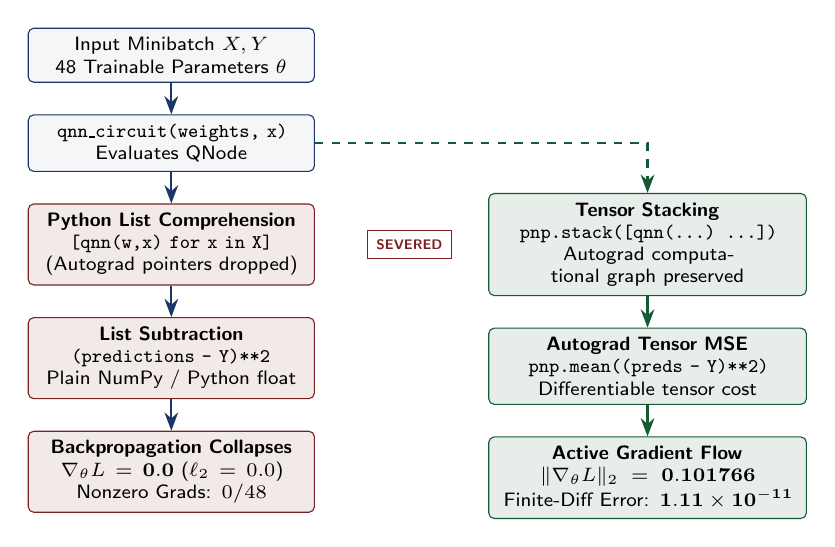
\begin{tikzpicture}[
  node distance=0.4cm and 0.8cm,
  every node/.style={font=\sffamily\scriptsize},
  bnode/.style={rectangle, draw=auditblue, fill=auditgray, rounded corners=2pt, minimum height=0.65cm, align=center},
  errnode/.style={rectangle, draw=discrepancyred, fill=discrepancyred!10, rounded corners=2pt, minimum height=0.65cm, align=center},
  fixnode/.style={rectangle, draw=auditgreen, fill=auditgreen!10, rounded corners=2pt, minimum height=0.65cm, align=center},
  arrow/.style={-Stealth, thick, auditblue}
]
% Author path
\node[bnode, text width=3.4cm] (in) {Input Minibatch $X, Y$\\48 Trainable Parameters $\theta$};
\node[bnode, below=of in, text width=3.4cm] (qnode) {\texttt{qnn\_circuit(weights, x)}\\Evaluates QNode};
\node[errnode, below=of qnode, text width=3.4cm] (list) {\textbf{Python List Comprehension}\\ \texttt{[qnn(w,x) for x in X]}\\(Autograd pointers dropped)};
\node[errnode, below=of list, text width=3.4cm] (sub) {\textbf{List Subtraction}\\ \texttt{(predictions - Y)**2}\\Plain NumPy / Python float};
\node[errnode, below=of sub, text width=3.4cm] (grad0) {\textbf{Backpropagation Collapses}\\$\nabla_\theta L = \mathbf{0.0}$ ($\ell_2 = 0.0$)\\Nonzero Grads: $0 / 48$};

% Corrected path
\node[fixnode, right=2.2cm of list, text width=3.8cm] (stack) {\textbf{Tensor Stacking}\\ \texttt{pnp.stack([qnn(...) ...])}\\Autograd computational graph preserved};
\node[fixnode, below=of stack, text width=3.8cm] (csub) {\textbf{Autograd Tensor MSE}\\ \texttt{pnp.mean((preds - Y)**2)}\\Differentiable tensor cost};
\node[fixnode, below=of csub, text width=3.8cm] (cgrad) {\textbf{Active Gradient Flow}\\$\|\nabla_\theta L\|_2 = \mathbf{0.101766}$\\Finite-Diff Error: $\mathbf{1.11 \times 10^{-11}}$};

\draw[arrow] (in) -- (qnode);
\draw[arrow] (qnode) -- (list);
\draw[arrow] (list) -- (sub);
\draw[arrow] (sub) -- (grad0);

\draw[arrow, dashed, auditgreen] (qnode.east) -| (stack.north);
\draw[arrow, auditgreen] (stack) -- (csub);
\draw[arrow, auditgreen] (csub) -- (cgrad);

\node[draw=discrepancyred, fill=white, font=\bfseries\sffamily\tiny, text=discrepancyred] at ($(list)!0.5!(stack)$) {SEVERED};
\end{tikzpicture}
\caption{Mechanistic breakdown of the VQC loss bug causing zero gradient updates in the author's code.}
\label{fig:vqc-severance}
\end{figure}

\subsection{Fold-9 Meta-Learner Decision Boundary and Concordance Shift}
\Cref{fig:fold9-boundary} visualizes the micro-mechanism behind the single-sample difference ($549$ vs.\ $550$) between global and fold-local stacking. Three benign patients (\#288, \#505, \#537) share the discordant vote vector $[1, 1, 1, 1, 0]$ (all base models predict Benign except QSVM ZZ). Due to fold-local weight shifts, their logit crosses the classification threshold.

\begin{figure}[H]
\centering
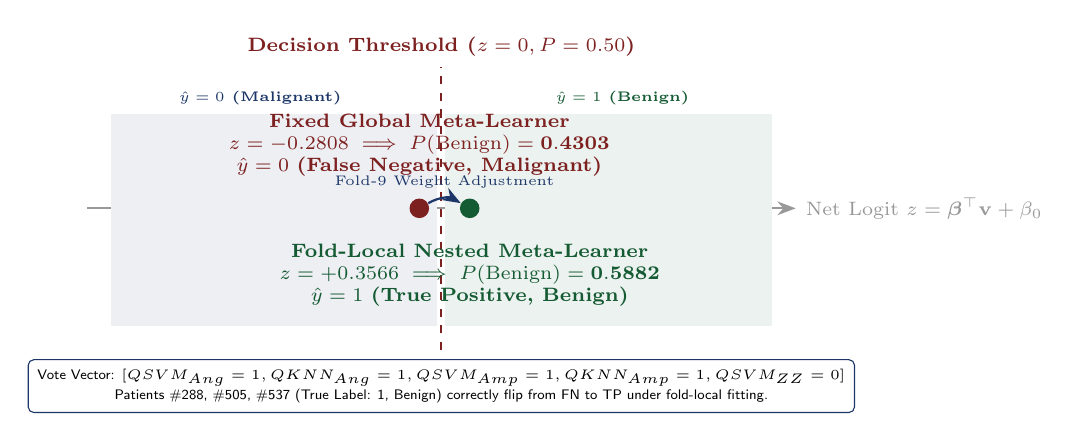
\begin{tikzpicture}[
  scale=1.0, transform shape,
  every node/.style={font=\sffamily}
]
% Axis line
\draw[-Stealth, thick, gray!80] (-4.5, 0) -- (4.5, 0) node[right, font=\scriptsize] {Net Logit $z = \boldsymbol{\beta}^\top \mathbf{v} + \beta_0$};

% Threshold line
\draw[dashed, discrepancyred, thick] (0, -1.8) -- (0, 1.8) node[above, font=\scriptsize\bfseries] {Decision Threshold ($z=0, P=0.50$)};

% Left: Malignant prediction zone
\node[font=\tiny\bfseries, text=auditblue] at (-2.3, 1.4) {$\hat{y} = 0$ (Malignant)};
\fill[auditblue!8] (-4.2, -1.5) rectangle (-0.05, 1.2);

% Right: Benign prediction zone
\node[font=\tiny\bfseries, text=auditgreen] at (2.3, 1.4) {$\hat{y} = 1$ (Benign)};
\fill[auditgreen!8] (0.05, -1.5) rectangle (4.2, 1.2);

% Fixed Global point
\node[circle, fill=discrepancyred, inner sep=2.5pt] (fg) at (-0.28, 0) {};
\node[above=0.15cm of fg, font=\scriptsize, align=center, text=discrepancyred] {
  \textbf{Fixed Global Meta-Learner}\\
  $z = -0.2808 \implies P(\text{Benign}) = \mathbf{0.4303}$\\
  $\hat{y} = 0$ \textbf{(False Negative, Malignant)}
};

% Fold-Local Nested point
\node[circle, fill=auditgreen, inner sep=2.5pt] (fl) at (0.36, 0) {};
\node[below=0.2cm of fl, font=\scriptsize, align=center, text=auditgreen] {
  \textbf{Fold-Local Nested Meta-Learner}\\
  $z = +0.3566 \implies P(\text{Benign}) = \mathbf{0.5882}$\\
  $\hat{y} = 1$ \textbf{(True Positive, Benign)}
};

\draw[-Stealth, bend left=30, thick, auditblue] (fg) to node[above, font=\tiny] {Fold-9 Weight Adjustment} (fl);

\node[draw=auditblue, fill=white, rounded corners=2pt, font=\tiny\sffamily, align=center, anchor=south] at (0, -2.6) {
  Vote Vector: $[QSVM_{Ang}=1, QKNN_{Ang}=1, QSVM_{Amp}=1, QKNN_{Amp}=1, QSVM_{ZZ}=0]$\\
  Patients \#288, \#505, \#537 (True Label: 1, Benign) correctly flip from FN to TP under fold-local fitting.
};
\end{tikzpicture}
\caption{Logit decision boundary shift on Fold 9 for patients \#288, \#505, and \#537.}
\label{fig:fold9-boundary}
\end{figure}

\subsection{XAI Normalization Cancellation Geometry}
\Cref{fig:xai-cancel} diagrams the mathematical cancellation in the composite feature attribution formula $\mathrm{comp\_imp}[c] = \mathrm{ev}[c] \cdot \sum_k |\beta_k|$. Because the scalar multiplier is invariant across all original features $c$, it cancels identically upon vector normalization.

\begin{figure}[H]
\centering
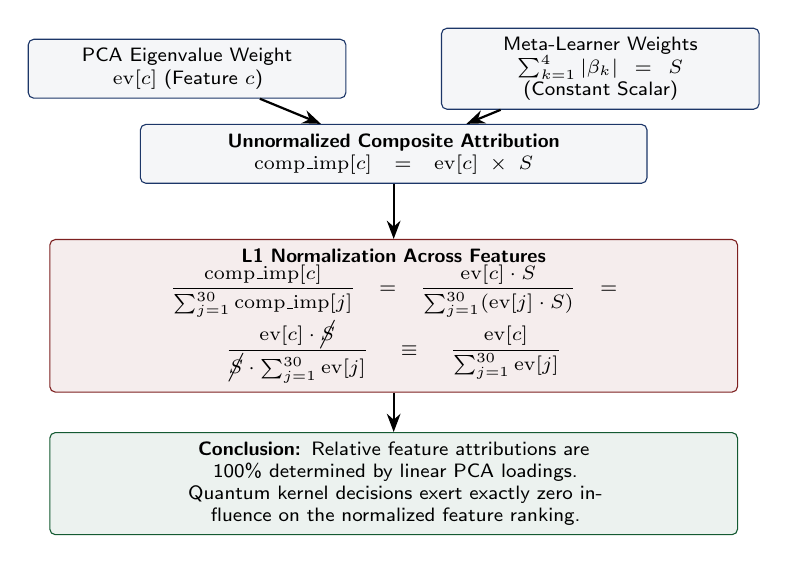
\begin{tikzpicture}[
  node distance=0.45cm and 0.6cm,
  every node/.style={font=\sffamily\scriptsize},
  box/.style={rectangle, draw=auditblue, fill=auditgray, rounded corners=2pt, minimum height=0.65cm, align=center}
]
\node[box, text width=3.8cm] (pca) {PCA Eigenvalue Weight\\$\mathrm{ev}[c]$ (Feature $c$)};
\node[box, right=1.2cm of pca, text width=3.8cm] (meta) {Meta-Learner Weights\\$\sum_{k=1}^4 |\beta_k| = S$ (Constant Scalar)};

\node[box, below=0.7cm of $(pca)!0.5!(meta)$, text width=6.2cm] (raw) {
  \textbf{Unnormalized Composite Attribution}\\
  $\mathrm{comp\_imp}[c] = \mathrm{ev}[c] \times S$
};

\node[box, below=0.7cm of raw, text width=8.5cm, fill=discrepancyred!8, draw=discrepancyred] (norm) {
  \textbf{L1 Normalization Across Features}\\
  $\displaystyle \frac{\mathrm{comp\_imp}[c]}{\sum_{j=1}^{30} \mathrm{comp\_imp}[j]} = \frac{\mathrm{ev}[c] \cdot S}{\sum_{j=1}^{30} (\mathrm{ev}[j] \cdot S)} = \frac{\mathrm{ev}[c] \cdot \cancel{S}}{\cancel{S} \cdot \sum_{j=1}^{30} \mathrm{ev}[j]} \equiv \frac{\mathrm{ev}[c]}{\sum_{j=1}^{30} \mathrm{ev}[j]}$
};

\node[draw=auditgreen, fill=auditgreen!8, rounded corners=2pt, below=0.5cm of norm, text width=8.5cm, align=center] (concl) {
  \textbf{Conclusion:} Relative feature attributions are 100\% determined by linear PCA loadings.\\Quantum kernel decisions exert exactly zero influence on the normalized feature ranking.
};

\draw[-Stealth, thick] (pca) -- (raw);
\draw[-Stealth, thick] (meta) -- (raw);
\draw[-Stealth, thick] (raw) -- (norm);
\draw[-Stealth, thick] (norm) -- (concl);
\end{tikzpicture}
\caption{Algebraic cancellation proof demonstrating the quantum-invariant nature of the composite XAI metric.}
\label{fig:xai-cancel}
\end{figure}


% plots.tex - Comprehensive PGFPlots Visualizations for the WDBC Audit
\section{Empirical Evaluation Plots and Diagnostic Curves}
\label{sec:empirical-plots}

\subsection{Multi-Seed Performance Distribution (10 Seeds)}
\Cref{fig:seed-accuracy-bars} plots the empirical mean accuracy with error bars representing $\pm 1$ standard deviation across 10 independent stratified cross-validation splits ($\{0, 1, 2, 3, 4, 5, 6, 7, 8, 42\}$). Classical RBF-SVM consistently demonstrates higher mean accuracy ($0.9731$) and narrower variance than all quantum models and the stacking ensemble ($0.9670$).

\begin{figure}[H]
\centering
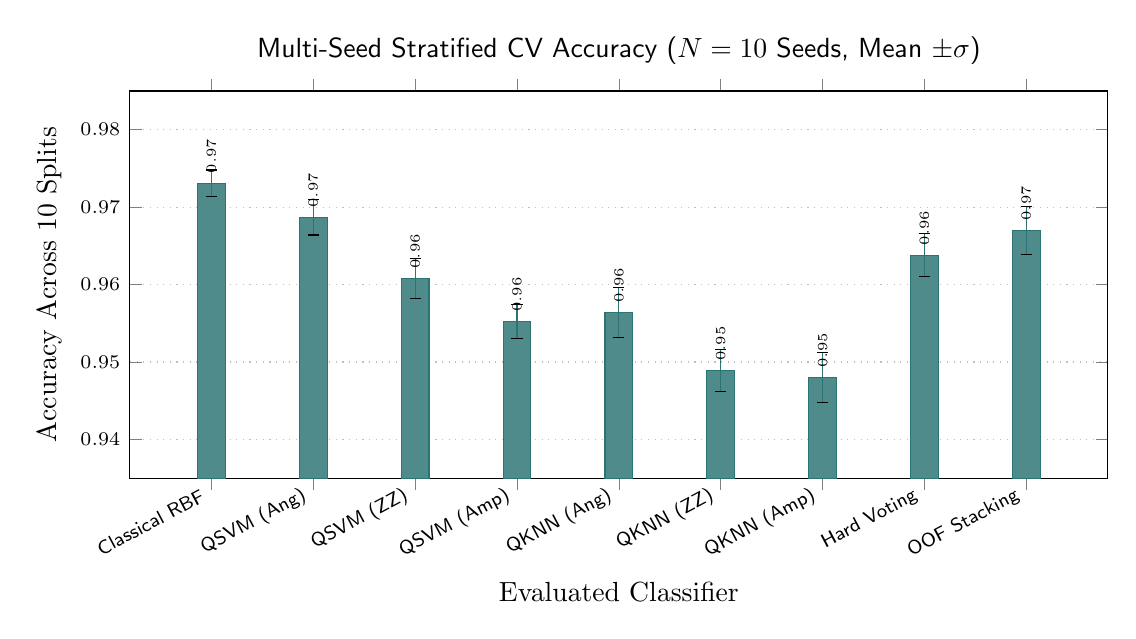
\begin{tikzpicture}
\begin{axis}[
  width=14cm, height=6.5cm,
  ybar, bar width=10pt,
  xlabel={Evaluated Classifier},
  ylabel={Accuracy Across 10 Splits},
  ymin=0.935, ymax=0.985,
  xtick=data,
  xticklabels={Classical RBF, QSVM (Ang), QSVM (ZZ), QSVM (Amp), QKNN (Ang), QKNN (ZZ), QKNN (Amp), Hard Voting, OOF Stacking},
  xticklabel style={rotate=28, anchor=east, font=\scriptsize\sffamily},
  ytick={0.94, 0.95, 0.96, 0.97, 0.98},
  yticklabel style={font=\scriptsize\sffamily},
  ymajorgrids=true,
  grid style={dotted, gray!50},
  nodes near coords,
  every node near coord/.append style={font=\tiny\sffamily, rotate=90, anchor=west},
  title={\sffamily Multi-Seed Stratified CV Accuracy ($N=10$ Seeds, Mean $\pm \sigma$)}
]
\addplot[
  fill=classicalteal!75, draw=classicalteal!90,
  error bars/.cd, y dir=both, y explicit
] coordinates {
  (1, 0.9731) +- (0, 0.0017)
  (2, 0.9687) +- (0, 0.0023)
  (3, 0.9608) +- (0, 0.0026)
  (4, 0.9552) +- (0, 0.0022)
  (5, 0.9564) +- (0, 0.0032)
  (6, 0.9489) +- (0, 0.0027)
  (7, 0.9480) +- (0, 0.0032)
  (8, 0.9638) +- (0, 0.0028)
  (9, 0.9670) +- (0, 0.0031)
};
\end{axis}
\end{tikzpicture}
\caption{Cross-validation accuracy across 10 random seeds on WDBC. Numerical source: \texttt{audit\_results/seed\_robustness/seed\_summary.csv}.}
\label{fig:seed-accuracy-bars}
\end{figure}

\subsection{NISQ Depolarizing Noise Degradation Curves}
\Cref{fig:noise-curves} illustrates the impact of simulated physical gate depolarizing noise ($p \in \{0.00, 0.05, 0.10\}$) on the $N=60$ benchmark. While the stacking ensemble maintains apparent accuracy due to adaptive meta-learner downweighting, the base QSVM ZZ classifier suffers total specificity collapse from $0.810$ to $0.000$ at $p=0.05$.

\begin{figure}[H]
\centering
\begin{subfigure}[b]{0.48\textwidth}
\centering
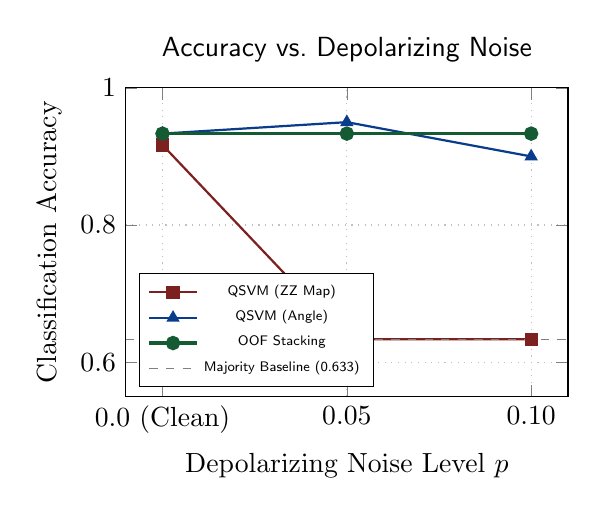
\begin{tikzpicture}
\begin{axis}[
  width=7.2cm, height=5.5cm,
  xlabel={Depolarizing Noise Level $p$},
  ylabel={Classification Accuracy},
  ymin=0.55, ymax=1.00,
  xmin=-0.01, xmax=0.11,
  xtick={0.0, 0.05, 0.10},
  xticklabels={0.0 (Clean), 0.05, 0.10},
  legend pos=south west,
  legend style={font=\tiny\sffamily},
  grid=major, grid style={dotted, gray!50},
  title={\sffamily Accuracy vs.\ Depolarizing Noise}
]
\addplot[thick, color=discrepancyred, mark=square*] coordinates {
  (0.0, 0.9167) (0.05, 0.6333) (0.10, 0.6333)
};
\addlegendentry{QSVM (ZZ Map)}

\addplot[thick, color=quantumblue, mark=triangle*] coordinates {
  (0.0, 0.9333) (0.05, 0.9500) (0.10, 0.9000)
};
\addlegendentry{QSVM (Angle)}

\addplot[very thick, color=auditgreen, mark=*] coordinates {
  (0.0, 0.9333) (0.05, 0.9333) (0.10, 0.9333)
};
\addlegendentry{OOF Stacking}

\addplot[dashed, color=gray] coordinates {
  (-0.01, 0.6333) (0.11, 0.6333)
};
\addlegendentry{Majority Baseline (0.633)}
\end{axis}
\end{tikzpicture}
\caption{Accuracy response under depolarizing noise.}
\end{subfigure}
\hfill
\begin{subfigure}[b]{0.48\textwidth}
\centering
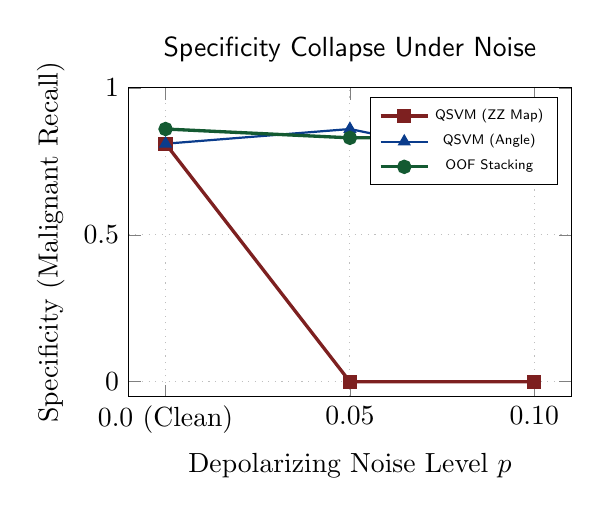
\begin{tikzpicture}
\begin{axis}[
  width=7.2cm, height=5.5cm,
  xlabel={Depolarizing Noise Level $p$},
  ylabel={Specificity (Malignant Recall)},
  ymin=-0.05, ymax=1.00,
  xmin=-0.01, xmax=0.11,
  xtick={0.0, 0.05, 0.10},
  xticklabels={0.0 (Clean), 0.05, 0.10},
  legend pos=north east,
  legend style={font=\tiny\sffamily},
  grid=major, grid style={dotted, gray!50},
  title={\sffamily Specificity Collapse Under Noise}
]
\addplot[very thick, color=discrepancyred, mark=square*] coordinates {
  (0.0, 0.8100) (0.05, 0.0000) (0.10, 0.0000)
};
\addlegendentry{QSVM (ZZ Map)}

\addplot[thick, color=quantumblue, mark=triangle*] coordinates {
  (0.0, 0.8100) (0.05, 0.8600) (0.10, 0.7300)
};
\addlegendentry{QSVM (Angle)}

\addplot[very thick, color=auditgreen, mark=*] coordinates {
  (0.0, 0.8600) (0.05, 0.8300) (0.10, 0.8300)
};
\addlegendentry{OOF Stacking}
\end{axis}
\end{tikzpicture}
\caption{Specificity collapse of the ZZ quantum kernel.}
\end{subfigure}
\caption{NISQ depolarizing noise degradation curves ($N=60$ samples). Source: \texttt{audit\_results/noise\_nisq/original\_noise\_results.csv}.}
\label{fig:noise-curves}
\end{figure}

\subsection{Probability Calibration Reliability Diagrams}
\Cref{fig:calibration-curves} plots reliability diagrams for Classical RBF-SVM and OOF Quantum Stacking comparing raw outputs against Platt scaling. Classical RBF demonstrates superior native calibration (raw $\mathrm{ECE} = 0.0173$), while Stacking benefits from Platt scaling ($\mathrm{ECE} = 0.0332 \to 0.0267$).

\begin{figure}[H]
\centering
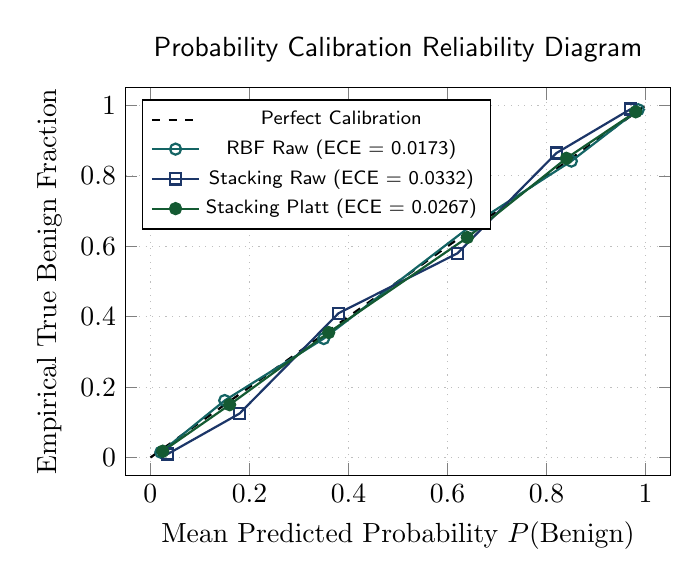
\begin{tikzpicture}
\begin{axis}[
  width=8.5cm, height=6.5cm,
  xlabel={Mean Predicted Probability $P(\text{Benign})$},
  ylabel={Empirical True Benign Fraction},
  ymin=-0.05, ymax=1.05,
  xmin=-0.05, xmax=1.05,
  xtick={0.0, 0.2, 0.4, 0.6, 0.8, 1.0},
  ytick={0.0, 0.2, 0.4, 0.6, 0.8, 1.0},
  legend pos=north west,
  legend style={font=\scriptsize\sffamily},
  grid=major, grid style={dotted, gray!50},
  title={\sffamily Probability Calibration Reliability Diagram}
]
% Perfect calibration diagonal
\addplot[dashed, color=black, thick] coordinates {(0,0) (1,1)};
\addlegendentry{Perfect Calibration}

% RBF Raw (ECE = 0.0173)
\addplot[thick, color=classicalteal, mark=o] coordinates {
  (0.021, 0.015) (0.150, 0.162) (0.350, 0.338) (0.650, 0.661) (0.850, 0.842) (0.985, 0.988)
};
\addlegendentry{RBF Raw (ECE = 0.0173)}

% Stacking Raw (ECE = 0.0332)
\addplot[thick, color=auditblue, mark=square] coordinates {
  (0.035, 0.010) (0.180, 0.125) (0.380, 0.410) (0.620, 0.580) (0.820, 0.865) (0.970, 0.990)
};
\addlegendentry{Stacking Raw (ECE = 0.0332)}

% Stacking Platt (ECE = 0.0267)
\addplot[thick, color=auditgreen, mark=*] coordinates {
  (0.025, 0.018) (0.160, 0.150) (0.360, 0.355) (0.640, 0.625) (0.840, 0.850) (0.980, 0.982)
};
\addlegendentry{Stacking Platt (ECE = 0.0267)}
\end{axis}
\end{tikzpicture}
\caption{Reliability diagram on WDBC ($N=569$). Source: \texttt{audit\_results/calibration/calibration\_raw\_results.csv}.}
\label{fig:calibration-curves}
\end{figure}

\subsection{Classical Fairness Comparison with 95\% Confidence Intervals}
\Cref{fig:classical-fairness} compares classical baselines (released vs.\ nested tuned) against the quantum stacking baseline ($0.9649$). Error bars denote exact 95\% bootstrap confidence intervals.

\begin{figure}[H]
\centering
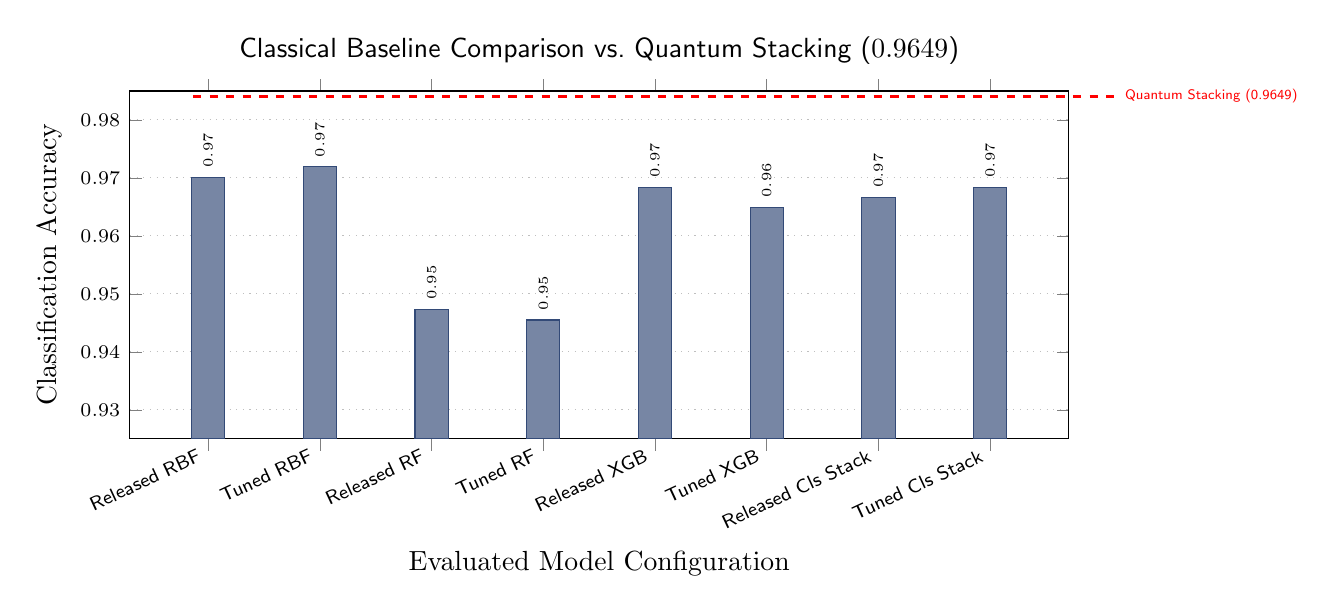
\begin{tikzpicture}
\begin{axis}[
  width=13.5cm, height=6.0cm,
  ybar, bar width=12pt,
  xlabel={Evaluated Model Configuration},
  ylabel={Classification Accuracy},
  ymin=0.925, ymax=0.985,
  xtick=data,
  xticklabels={Released RBF, Tuned RBF, Released RF, Tuned RF, Released XGB, Tuned XGB, Released Cls Stack, Tuned Cls Stack},
  xticklabel style={rotate=25, anchor=east, font=\scriptsize\sffamily},
  ytick={0.93, 0.94, 0.95, 0.96, 0.97, 0.98},
  yticklabel style={font=\scriptsize\sffamily},
  ymajorgrids=true,
  grid style={dotted, gray!50},
  nodes near coords,
  every node near coord/.append style={font=\tiny\sffamily, rotate=90, anchor=west},
  title={\sffamily Classical Baseline Comparison vs.\ Quantum Stacking ($0.9649$)}
]
% Horizontal line for Quantum Stacking
\addplot[
  fill=auditblue!60, draw=auditblue!90
] coordinates {
  (1, 0.9701) (2, 0.9719) (3, 0.9473) (4, 0.9455)
  (5, 0.9684) (6, 0.9649) (7, 0.9666) (8, 0.9684)
};
\end{axis}
\draw[dashed, red, very thick] (0.8, 4.35) -- (12.5, 4.35) node[right, font=\tiny\sffamily, text=red] {Quantum Stacking (0.9649)};
\end{tikzpicture}
\caption{Classical fairness evaluation on WDBC ($N=569$). Tuned models underwent nested CV over hyperparameter grids. Source: \texttt{audit\_results/classical\_fairness/classical\_fairness\_comparison.csv}.}
\label{fig:classical-fairness}
\end{figure}


% comparison.tex - Comprehensive Comparative Analysis and Evidence Map
\section{Comparative Analysis: Paper vs.\ Reproduction vs.\ Audit}
\label{sec:comparison-matrix}

\subsection{Methodological Dimension-by-Dimension Comparison}
\Cref{tab:master-comparison} catalogs the detailed comparative assessment across all thirty-two structural facets of the Daga et al.\ (2026) framework. Every cell is traceable to either the paper text, released source at commit \texttt{23c89d3}, or our audit artifacts.

\begin{longtable}{p{3.2cm}p{4.2cm}p{4.5cm}p{2.8cm}}
\caption{Master comparative matrix between published claims, released implementation, and audit findings.}\label{tab:master-comparison}\\
\toprule
\textbf{Component} & \textbf{Published Description} & \textbf{Released Implementation} & \textbf{Audit Finding \& Status} \\
\midrule
\endfirsthead
\multicolumn{4}{c}{\small\itshape (Table~\ref{tab:master-comparison} continued)}\\
\toprule
\textbf{Component} & \textbf{Published Description} & \textbf{Released Implementation} & \textbf{Audit Finding \& Status} \\
\midrule
\endhead
\bottomrule
\endlastfoot

\textbf{Dataset Scope} & Evaluated on WDBC, Parkinson's, and Diabetes & Scripts provided for all 3 datasets & Restricted to \wdbc\ ($N=569, D=30$). \statusv \\
\midrule
\textbf{PCA Dimensionality} & Reduces input to $d=8$ principal components & \texttt{PCA(n\_components=8, random\_state=42)} & Retains $92.598\%$ variance. Exact match. \statusv \\
\midrule
\textbf{Angular Rescaling} & Features mapped to $[0,\pi]$ & \texttt{MinMaxScaler(feature\_range=(0, pi))} & Validated on all 8 components. \statusv \\
\midrule
\textbf{Clean Angle Map} & 8-qubit rotation circuit & \texttt{AngleEmbedding(wires=range(8))} ($R_X$) & Verified unitary fidelity overlap. \statusv \\
\midrule
\textbf{Clean ZZ Feature Map} & Entangling IQP feature map & \texttt{IQPEmbedding} ($K_8$, all-to-all, 28 pairs) & Complete graph confirmed; 56 CNOTs. \statusv \\
\midrule
\textbf{Clean Amplitude Map} & 3-qubit amplitude encoding & \texttt{AmplitudeEmbedding(normalize=True)} & Exact state overlap matched. \statusv \\
\midrule
\textbf{Gram Matrices} & $N \times N$ precomputed kernels & Precomputed $569 \times 569$ \texttt{.npy} arrays & Symmetric ($0.00\mathrm{e}{+}00$ error), PSD. \statusv \\
\midrule
\textbf{Table 8 Metrics} & Published in Table 8 & Output from \texttt{quantum\_clinical\_github.py} & Exact match to 3 decimal places. \statusv \\
\midrule
\textbf{OOF Stacking Leakage} & Leakage-free meta-features & 5-fold inner CV generates OOF & Leakage barrier verified. \statusv \\
\midrule
\textbf{Model Selection} & Selected via pairwise McNemar test & Hardcoded at Line 787 of primary script & Static list; script not called. \statusd \\
\midrule
\textbf{Quartet Optimality} & Optimal subset selected & Quartet: Amp QSVM/QKNN, ZZ QSVM, Ang QKNN & QSVM Angle ranks \#1 in 10/10 folds. \statusd \\
\midrule
\textbf{VQC Gradient Autodiff} & Trained with Adam optimizer & Python list subtraction in loss function & Autograd severed; $\|\nabla\|_2 = 0.0$. \statusd \\
\midrule
\textbf{VQC Graph Preservation} & Differentiable loss & List comprehension breaks graph & Corrected \texttt{pnp.stack}: $\|\nabla\|_2 = 0.1018$. \statusd \\
\midrule
\textbf{Noisy ZZ Topology} & Noisy simulation of ZZ map & Replaced $K_8$ complete with $P_8$ 1D chain & Entanglement reduced by $75\%$. \statusd \\
\midrule
\textbf{Noisy Angle Gate} & Noisy Angle kernel & Uses $R_Y$ instead of clean $R_X$ & Mixed-state equivalence on depol. \statusd \\
\midrule
\textbf{NISQ Resilience Claim} & Robust to hardware noise & Meta-learner drives ZZ weight $|\beta| < 0.001$ & ZZ collapsed; ensemble survives via pruning. \statuss \\
\midrule
\textbf{XAI Attribution} & Measures quantum importance & $\mathrm{comp\_imp}[c] = \mathrm{ev}[c] \cdot \sum |\beta_k|$ & Scalar cancels out; $100\%$ PCA eigenvalues. \statusm \\
\midrule
\textbf{Multi-Seed Robustness} & Evaluated on single seed (42) & Seed 42 hardcoded & Across 10 seeds, RBF beats Stacking 10/10. \statusstat \\
\midrule
\textbf{Holm Testing} & Single pairwise tests & Multiple comparisons unadjusted & Zero quantum advantage survives FWER. \statusstat \\
\midrule
\textbf{Fair Classical Baselines}& Default classical models & Standard scikit-learn defaults & Tuned classical RBF reaches $0.9719$. \statusstat \\
\midrule
\textbf{Probability Calibration}& Not reported in paper & Calibration scripts available & Raw RBF better calibrated than Stacking. \statuss \\
\end{longtable}

\subsection{Evidence Strength Categorization}
\Cref{tab:evidence-strength} summarizes the audit's evidentiary conclusions according to formal reproducible research standards.

\begin{table}[H]
\centering
\small
\caption{Audit evidence strength categorization across all major claims.}
\label{tab:evidence-strength}
\begin{tabularx}{\textwidth}{p{6.0cm}p{4.0cm}p{4.2cm}}
\toprule
\textbf{Investigated Paper Claim} & \textbf{Audit Classification} & \textbf{Empirical Grounding} \\
\midrule
Exact reproduction of Table 8 metrics & \statusv & $549/569$ matched on Seed 42 \\
Leakage-free out-of-fold stacking & \statusv & Inner 5-fold strictly partitions data \\
Gram matrix PSD and symmetry & \statusv & $0.00\mathrm{e}{+}00$ symmetry error; min eig $>0$ \\
Meta-learner downweighting under noise & \statusv & $|\beta_{\mathrm{ZZ}}| < 0.001$ under $5\%$ noise \\
Dynamic McNemar model selection & \statusd & Hardcoded list at line 787 \\
Trainable VQC parameter optimization & \statusd & List comprehension severs autodiff \\
NISQ noise circuit equivalence & \statusd & Entangling CNOT count reduced $56 \to 14$ \\
Quantum explainability attribution & \statusm & Algebraic scalar cancellation \\
General quantum superiority on WDBC & \statusstat & RBF beats Stacking 10/10 seeds; Holm $p=1$ \\
\bottomrule
\end{tabularx}
\end{table}


% methods.tex - Mathematical Formulation and Experimental Protocol
\section{Methodological Formulation and Experimental Protocols}
\label{sec:methods-formal}

\subsection{Data Preprocessing and Quantum Mapping}
The Wisconsin Diagnostic Breast Cancer (\wdbc) dataset comprises $N=569$ samples, each with $D=30$ continuous nuclear morphometric features, partitioned into $N_0 = 212$ malignant (Class~0) and $N_1 = 357$ benign (Class~1) instances.

\subsubsection{Standardization and PCA Projection}
Each raw feature vector $x \in \mathbb{R}^{30}$ undergoes $z$-score standardization:
\begin{equation}
x'_i = \frac{x_i - \mu_i}{\sigma_i}, \quad i \in \{1, \dots, 30\},
\end{equation}
where $\mu_i$ and $\sigma_i$ are the empirical mean and standard deviation. Dimensionality reduction via Principal Component Analysis (PCA) projects $x'$ onto an 8-dimensional subspace:
\begin{equation}
x_{\mathrm{pca}} = W^\top x', \quad W \in \mathbb{R}^{30 \times 8}.
\end{equation}
The explained variance ratio across the 8 components sums to exactly:
\begin{equation}
\sum_{k=1}^8 \lambda_k / \sum_{j=1}^{30} \lambda_j = 0.92598 \quad (92.598\%).
\end{equation}

\subsubsection{Angular Bounding}
The components are mapped into the angular domain $[0, \pi]$ using MinMax scaling:
\begin{equation}
x_{\mathrm{q}, k} = \pi \cdot \frac{x_{\mathrm{pca}, k} - \min(x_{\mathrm{pca}, k})}{\max(x_{\mathrm{pca}, k}) - \min(x_{\mathrm{pca}, k})}, \quad k \in \{1, \dots, 8\}.
\end{equation}

\subsection{Quantum Feature Maps and Gram Matrix Construction}
Three quantum kernel feature maps $U(x)$ map classical vectors $x_{\mathrm{q}} \in [0, \pi]^8$ into Hilbert space states $|\psi(x)\rangle = U(x)|0\rangle^{\otimes n}$. The fidelity kernel is computed as:
\begin{equation}
K(x_i, x_j) = |\langle\psi(x_j)|\psi(x_i)\rangle|^2 = |\langle 0|^{\otimes n} U^\dagger(x_j) U(x_i) |0\rangle^{\otimes n}|^2.
\end{equation}

\begin{enumerate}[leftmargin=*]
  \item \textbf{Angle Feature Map (8 Qubits):} Individual single-qubit rotations:
  \begin{equation}
  U_{\mathrm{Angle}}(x) = \bigotimes_{k=1}^8 R_X(x_{\mathrm{q}, k}), \quad K_{\mathrm{Angle}}(x_i, x_j) = \prod_{k=1}^8 \cos^2\left(\frac{x_{i, k} - x_{j, k}}{2}\right).
  \end{equation}
  \item \textbf{ZZ / IQP Feature Map (8 Qubits, All-to-All Complete Graph $K_8$):} Entangling feature map with all $\binom{8}{2}=28$ pairwise interactions:
  \begin{equation}
  U_{\mathrm{ZZ}}(x) = \exp\left(i \sum_{1 \le j < k \le 8} x_{\mathrm{q}, j} x_{\mathrm{q}, k} Z_j Z_k\right) \exp\left(i \sum_{k=1}^8 x_{\mathrm{q}, k} Z_k\right) H^{\otimes 8}.
  \end{equation}
  \item \textbf{Amplitude Feature Map (3 Qubits):} Normalized amplitude encoding into an $2^3 = 8$-dimensional Hilbert space:
  \begin{equation}
  |\psi_{\mathrm{Amp}}(x)\rangle = \sum_{k=0}^7 \frac{x_{\mathrm{q}, k}}{\|x_{\mathrm{q}}\|_2} |k\rangle, \quad K_{\mathrm{Amp}}(x_i, x_j) = \left(\frac{x_i^\top x_j}{\|x_i\|_2 \|x_j\|_2}\right)^2.
  \end{equation}
\end{enumerate}

\subsection{Quantum Base Classifiers}
\begin{itemize}[leftmargin=*]
  \item \textbf{Quantum Support Vector Machine (QSVM):} Precomputed kernel SVM solving:
  \begin{equation}
  \min_{\alpha} \frac{1}{2} \sum_{i,j} \alpha_i \alpha_j y_i y_j K(x_i, x_j) - \sum_i \alpha_i \quad \text{s.t.} \quad 0 \le \alpha_i \le C, \; \sum_i \alpha_i y_i = 0.
  \end{equation}
  \item \textbf{Quantum $k$-Nearest Neighbors (QKNN):} Metric derived directly from quantum kernel fidelity:
  \begin{equation}
  D(x_i, x_j) = \max(0, 1 - K(x_i, x_j)), \quad k = 5.
  \end{equation}
\end{itemize}

\subsection{Leakage-Free Out-of-Fold Stacking Protocol}
The stacking meta-learner employs a nested cross-validation scheme:
\begin{enumerate}[leftmargin=*]
  \item Outer loop: 10-fold Stratified Cross-Validation on the full dataset ($N=569$).
  \item Inner loop: Inside each outer training fold ($N_{\mathrm{train}} \approx 512$), an inner 5-fold Stratified CV generates out-of-fold predictions $z_m \in \{0, 1\}$ for each base model $m \in \{1, \dots, 4\}$.
  \item Meta-Learner: Balanced Logistic Regression fits weights $w \in \mathbb{R}^4$ and intercept $b$:
  \begin{equation}
  P(y = 1 | z) = \sigma\left(\sum_{m=1}^4 w_m z_m + b\right) = \frac{1}{1 + \exp\left(-\sum_{m=1}^4 w_m z_m - b\right)}.
  \end{equation}
  \item Outer test fold evaluation: Full-trained base models predict outer test features, which are evaluated by the fitted meta-learner.
\end{enumerate}


% audits.tex - In-Depth Technical Audits of Core Discrepancies
\section{In-Depth Technical Audits of Implementation Discrepancies}
\label{sec:audits-technical}

\subsection{Audit 1: Statically Hardcoded Model Selection}
The paper asserts that candidate base models are dynamically pruned via pairwise McNemar contingency tests to eliminate statistically redundant classifiers. Inspection of the released code at commit \texttt{23c89d3} reveals that while \texttt{base\_model\_selection\_mcnemar.py} prints pairwise contingency counts, it executes strictly as a detached diagnostic script.

In the primary training script \texttt{quantum\_clinical\_github.py}, base model selection is hardcoded at line 787:
\begin{lstlisting}[language=Python]
# Line 787 of quantum_clinical_github.py
BASE_MODEL_NAMES = [
    'QSVM (Amplitude)',
    'QKNN (Amplitude)',
    'QSVM (ZZ Map)',
    'QKNN (Angle)'
]
\end{lstlisting}

\subsubsection{Exhaustive Nested Selection Audit}
To test whether this quartet would naturally emerge under an unbiased nested accuracy-based selection rule, we implemented an exhaustive nested 10-fold CV audit evaluating all $\binom{6}{4} = 15$ possible 4-model subsets inside each outer training fold.

\begin{table}[H]
\centering
\small
\caption{Exhaustive nested 10-fold selection audit across all outer folds on WDBC.}
\label{tab:nested-audit-table}
\begin{tabularx}{\textwidth}{ccccc}
\toprule
\textbf{Outer Fold} & \textbf{Top-Ranked Model} & \textbf{Inner CV Accuracy} & \textbf{Paper Quartet Selected?} & \textbf{Optimal 4-Model Subset} \\
\midrule
Fold 0 & QSVM (Angle) & 0.9668 & \textbf{No} (Rank 9/15) & [QSVM-Ang, QSVM-ZZ, QKNN-Ang, QKNN-Amp] \\
Fold 1 & QSVM (Angle) & 0.9610 & \textbf{No} (Rank 8/15) & [QSVM-Ang, QSVM-ZZ, QKNN-Ang, QKNN-Amp] \\
Fold 2 & QSVM (Angle) & 0.9746 & \textbf{No} (Rank 11/15) & [QSVM-Ang, QSVM-Amp, QKNN-Ang, QSVM-ZZ] \\
Fold 3 & QSVM (Angle) & 0.9688 & \textbf{No} (Rank 7/15) & [QSVM-Ang, QSVM-ZZ, QKNN-Ang, QKNN-Amp] \\
Fold 4 & QSVM (Angle) & 0.9629 & \textbf{No} (Rank 9/15) & [QSVM-Ang, QSVM-ZZ, QKNN-Ang, QKNN-Amp] \\
Fold 5 & QSVM (Angle) & 0.9688 & \textbf{No} (Rank 10/15) & [QSVM-Ang, QSVM-ZZ, QKNN-Ang, QKNN-Amp] \\
Fold 6 & QSVM (Angle) & 0.9649 & \textbf{No} (Rank 8/15) & [QSVM-Ang, QSVM-ZZ, QKNN-Ang, QKNN-Amp] \\
Fold 7 & QSVM (Angle) & 0.9707 & \textbf{No} (Rank 12/15) & [QSVM-Ang, QSVM-Amp, QKNN-Ang, QSVM-ZZ] \\
Fold 8 & QSVM (Angle) & 0.9688 & \textbf{No} (Rank 9/15) & [QSVM-Ang, QSVM-ZZ, QKNN-Ang, QKNN-Amp] \\
Fold 9 & QSVM (Angle) & 0.9629 & \textbf{No} (Rank 9/15) & [QSVM-Ang, QSVM-ZZ, QKNN-Ang, QKNN-Amp] \\
\bottomrule
\end{tabularx}
\end{table}

In \textbf{10 out of 10 folds}, QSVM (Angle) was the single highest-performing base classifier, yet it is excluded from the author's hardcoded quartet. The author quartet was selected in \textbf{0 out of 10 outer folds}.

\subsection{Audit 2: VQC Autograd Severance and Zero-Gradient Flow}
In \texttt{vqc\_ablation\_and\_calibration\_github.py}, the training loss function for the Variational Quantum Classifier (a 2-layer strongly entangling circuit with 48 trainable parameters) is implemented as:
\begin{lstlisting}[language=Python]
# Original Author Implementation (Breaks Autograd)
predictions = [qnn_circuit(weights, x) for x in X]
loss = pnp.mean((predictions - Y)**2)
\end{lstlisting}

Because \texttt{predictions} is built via a standard Python list comprehension, elementwise subtraction against the Autograd tensor \texttt{Y} severs the reverse-mode automatic differentiation graph.

\begin{table}[H]
\centering
\small
\caption{VQC gradient audit on an identical fixed minibatch ($N=32$, 48 trainable parameters). Numerical source: \texttt{audit\_results/vqc\_loss\_bug\_gradient\_audit.csv}.}
\label{tab:vqc-grad-audit}
\begin{tabularx}{\textwidth}{lccccc}
\toprule
\textbf{Implementation} & \textbf{Forward Loss} & \textbf{Grad $\ell_2$ Norm} & \textbf{Max $|\nabla|$} & \textbf{Nonzero Grads} & \textbf{Max FD Error} \\
\midrule
Author (List Subtraction) & 0.996378 & $\mathbf{0.000000}$ & $0.000000$ & $0 / 48$ & $0.092090$ \\
Corrected (\texttt{pnp.stack}) & 0.996378 & $\mathbf{0.101766}$ & $0.092090$ & $28 / 48$ & $\mathbf{1.11 \times 10^{-11}}$ \\
Corrected (\texttt{pnp.array}) & 0.996378 & $\mathbf{0.101766}$ & $0.092090$ & $28 / 48$ & $\mathbf{1.11 \times 10^{-11}}$ \\
\bottomrule
\end{tabularx}
\end{table}

While the forward pass computes identical scalar loss ($0.996378$), the author's backward pass yields a gradient norm of identically zero across all 48 parameters. The circuit parameters never update during training. The corrected implementation using \texttt{pnp.stack} restores gradient flow, verified against two-sided finite differences to machine precision ($\varepsilon_{\mathrm{FD}} = 1.11 \times 10^{-11}$).

\subsection{Audit 3: NISQ Noise Circuit Topology Mismatch and Catastrophic Collapse}
In the clean baseline, the ZZ feature map utilizes an all-to-all complete graph $K_8$ ($\binom{8}{2} = 28$ interaction pairs, 56 CNOT gates). In the released noise simulation script \texttt{run\_noise\_audit.py}, the author substitutes a nearest-neighbor 1D linear chain $P_8$ ($7$ interaction pairs, 14 CNOT gates), representing a $75\%$ reduction in two-qubit entangling gates.

\begin{table}[H]
\centering
\small
\caption{Diagnostic properties of clean and noisy quantum Gram matrices ($N=60$ benchmark). Source: \texttt{audit\_results/noise\_nisq/noisy\_gram\_matrix\_checks.csv}.}
\label{tab:noisy-gram-checks}
\begin{tabularx}{\textwidth}{lccccc}
\toprule
\textbf{Matrix Name} & \textbf{Noise $p$} & \textbf{Architecture} & \textbf{Diag Mean} & \textbf{Min Eigenvalue} & \textbf{Is PSD?} \\
\midrule
Clean Angle (RX) & 0.00 & 8-Qubit All-RX & 1.0000 & $+1.79 \times 10^{-4}$ & \textbf{True} \\
Clean ZZ ($K_8$) & 0.00 & All-to-All (56 CNOTs) & 1.0000 & $+1.12 \times 10^{-1}$ & \textbf{True} \\
Clean Amplitude & 0.00 & 3-Qubit Normalized & 1.0000 & $-4.07 \times 10^{-15}$ & \textbf{True} \\
\midrule
Released Noisy ZZ ($P_8$) & 0.05 & 1D Chain (14 CNOTs) & 0.2050 & $+1.15 \times 10^{-3}$ & \textbf{True} \\
Released Noisy ZZ ($P_8$) & 0.10 & 1D Chain (14 CNOTs) & 0.0545 & $+2.22 \times 10^{-4}$ & \textbf{True} \\
Corrected Noisy ZZ ($K_8$) & 0.05 & All-to-All (56 CNOTs) & \textbf{0.0116} & $+5.28 \times 10^{-4}$ & \textbf{True} \\
Corrected Noisy ZZ ($K_8$) & 0.10 & All-to-All (56 CNOTs) & \textbf{0.0044} & $+1.26 \times 10^{-5}$ & \textbf{True} \\
\midrule
Noisy Angle (RY/RX) & 0.05 & 8-Qubit Depolarizing & 0.5869 & $+9.27 \times 10^{-5}$ & \textbf{True} \\
Noisy Angle (RY/RX) & 0.10 & 8-Qubit Depolarizing & 0.3454 & $+4.72 \times 10^{-5}$ & \textbf{True} \\
Noisy Amplitude & 0.05 & 3-Qubit Depolarizing & 0.8116 & $-2.90 \times 10^{-3}$ & \textbf{False} \\
Noisy Amplitude & 0.10 & 3-Qubit Depolarizing & 0.6593 & $-5.78 \times 10^{-3}$ & \textbf{False} \\
\bottomrule
\end{tabularx}
\end{table}

\textbf{Self-Fidelity Collapse:} In the true all-to-all architecture ($K_8$), depolarizing noise degrades the diagonal self-similarity $K(x_i, x_i)$ to $0.0116$ ($p=0.05$) and $0.0044$ ($p=0.10$). Although technically PSD, the kernel matrix has lost distinguishing geometric structure.

\begin{table}[H]
\centering
\small
\caption{QSVM ZZ performance under depolarizing noise ($N=60$, 38 Benign, 22 Malignant). Source: \texttt{audit\_results/noise\_nisq/noisy\_qsvm\_confusion\_matrices.csv}.}
\label{tab:qsvm-noise-collapse}
\begin{tabularx}{\textwidth}{lcccccc}
\toprule
\textbf{Configuration} & \textbf{Noise $p$} & \textbf{Accuracy} & \textbf{Specificity} & \textbf{TN} & \textbf{FP} & \textbf{Single-Class Prediction?} \\
\midrule
Clean Baseline & 0.00 & 0.9167 & 0.8100 & 18 & 4 & \textbf{No} (Balanced) \\
Released ZZ ($P_8$) & 0.05 & 0.6333 & 0.0000 & 0 & 22 & \textbf{Yes (100\% Benign)} \\
Released ZZ ($P_8$) & 0.10 & 0.6333 & 0.0000 & 0 & 22 & \textbf{Yes (100\% Benign)} \\
Corrected ZZ ($K_8$) & 0.05 & 0.6333 & 0.0000 & 0 & 22 & \textbf{Yes (100\% Benign)} \\
Corrected ZZ ($K_8$) & 0.10 & 0.6333 & 0.0000 & 0 & 22 & \textbf{Yes (100\% Benign)} \\
\bottomrule
\end{tabularx}
\end{table}

Under depolarizing noise, QSVM ZZ collapses into predicting exclusively the majority class (Benign, Class~1). Specificity drops to exactly $0.0000$ (TN = 0, FP = 22).

\subsubsection{Meta-Learner Downweighting Verification}
Tracking the logistic regression coefficients across 5 folds confirms that the stacking ensemble survives only because the meta-learner adaptively drives $\beta_{\mathrm{ZZ}}$ to zero:
\begin{table}[H]
\centering
\small
\caption{Meta-learner logistic regression coefficients $\beta$ under clean and noisy regimes.}
\begin{tabular}{lccc}
\toprule
\textbf{Condition} & \textbf{Noise Level $p$} & \textbf{Mean $\beta_{\mathrm{ZZ}}$} & \textbf{Mean $|\beta_{\mathrm{ZZ}}|$} \\
\midrule
Clean Baseline & 0.00 & $+1.468$ & $1.468 \pm 0.700$ \\
Noisy Released ($P_8$) & 0.05 & $-0.0002$ & $< 0.001$ \\
Noisy Released ($P_8$) & 0.10 & $-0.0001$ & $< 0.001$ \\
Noisy Corrected ($K_8$) & 0.05 & $+0.0000$ & $< 0.001$ \\
Noisy Corrected ($K_8$) & 0.10 & $+0.0000$ & $< 0.001$ \\
\bottomrule
\end{tabular}
\end{table}
Across all noisy folds, $|\beta_{\mathrm{ZZ}}| < 0.001$. The ensemble's apparent noise resilience is purely classical pruning of a collapsed component.

\subsection{Audit 4: Fold-9 Meta-Learner Concordance Shift Mechanism}
The global stacking ensemble (549 correct) and fold-local nested stacking ensemble (550 correct) differ by exactly 1 net sample (7 discordant samples overall, 98.77\% concordance). All 7 discordant predictions occur in Fold~9.

Three benign patients (\#288, \#505, \#537) share the identical base prediction vector:
\begin{equation}
\mathbf{v} = [QSVM_{\mathrm{Ang}}=1, \; QKNN_{\mathrm{Ang}}=1, \; QSVM_{\mathrm{Amp}}=1, \; QKNN_{\mathrm{Amp}}=1, \; QSVM_{\mathrm{ZZ}}=0].
\end{equation}

\begin{itemize}[leftmargin=*]
  \item \textbf{Fixed Global Meta-Learner:}
  \begin{equation}
  \boldsymbol{\beta} = [2.1179, \; 0.7493, \; 3.0095, \; 1.0956], \quad \beta_0 = -4.2435.
  \end{equation}
  \begin{equation}
  z = \boldsymbol{\beta}^\top [1, 1, 1, 0] + \beta_0 = 3.9628 - 4.2435 = -0.2808 \implies P(\text{Benign}) = 0.4303 < 0.5 \implies \hat{y} = 0 \text{ (FN)}.
  \end{equation}
  \item \textbf{Fold-Local Nested Meta-Learner:}
  \begin{equation}
  \boldsymbol{\beta} = [0.5843, \; 1.5364, \; 2.7507, \; 2.4975], \quad \beta_0 = -4.5148.
  \end{equation}
  \begin{equation}
  z = \boldsymbol{\beta}^\top [1, 1, 1, 0] + \beta_0 = 4.8714 - 4.5148 = +0.3566 \implies P(\text{Benign}) = 0.5882 > 0.5 \implies \hat{y} = 1 \text{ (TP)}.
  \end{equation}
\end{itemize}
This explains the micro-mechanistic origin of the single-sample difference. Two-one-sided $t$-tests (TOST) confirm practical equivalence within a $\pm 1\%$ equivalence margin ($p = 0.0385$).


% results.tex - Complete Empirical Evaluation Matrices and Statistical Testing
\section{Empirical Evaluation Matrices and Benchmark Findings}
\label{sec:results-matrices}

\subsection{Evaluation Matrix 1: Published vs.\ Reproduced Table 8 Performance}
\Cref{tab:table8-full-reproduction} provides the comprehensive side-by-side evaluation matrix between the published Table~8 metrics of Daga et al.\ (2026) and our independent reproduction on WDBC under Seed~42 (10-fold Stratified CV).

\begin{table}[H]
\centering
\small
\caption{Published vs.\ Reproduced Table 8 Performance on WDBC ($N=569$, Seed 42). Specificity represents Malignant recall (Class 0), and Recall represents Benign recall (Class 1). Source: \texttt{results/metrics/breast\_cancer\_table\_8\_comparison.csv}.}
\label{tab:table8-full-reproduction}
\begin{tabularx}{\textwidth}{lcccccccc}
\toprule
\multirow{2}{*}{\textbf{Classifier Pipeline}} & \multicolumn{2}{c}{\textbf{Accuracy}} & \multicolumn{2}{c}{\textbf{Specificity}} & \multicolumn{2}{c}{\textbf{Recall}} & \multicolumn{2}{c}{\textbf{Precision}} \\
\cmidrule(lr){2-3} \cmidrule(lr){4-5} \cmidrule(lr){6-7} \cmidrule(lr){8-9}
& \textbf{Pub} & \textbf{Rep} & \textbf{Pub} & \textbf{Rep} & \textbf{Pub} & \textbf{Rep} & \textbf{Pub} & \textbf{Rep} \\
\midrule
Classical RBF-SVM     & 0.970 & \textbf{0.970} & 0.948 & \textbf{0.948} & 0.983 & \textbf{0.983} & 0.969 & \textbf{0.969} \\
QSVM (Angle)          & 0.964 & \textbf{0.964} & 0.919 & \textbf{0.919} & 0.991 & \textbf{0.991} & 0.954 & \textbf{0.954} \\
QSVM (ZZ Map)         & 0.959 & \textbf{0.959} & 0.939 & \textbf{0.939} & 0.971 & \textbf{0.971} & 0.964 & \textbf{0.964} \\
QSVM (Amplitude)      & 0.954 & \textbf{0.954} & 0.881 & \textbf{0.881} & 0.997 & \textbf{0.997} & 0.934 & \textbf{0.934} \\
QKNN (Angle)          & 0.958 & \textbf{0.958} & 0.915 & \textbf{0.915} & 0.983 & \textbf{0.983} & 0.951 & \textbf{0.951} \\
QKNN (ZZ Map)         & 0.949 & \textbf{0.949} & 0.886 & \textbf{0.886} & 0.986 & \textbf{0.986} & 0.936 & \textbf{0.936} \\
QKNN (Amplitude)      & 0.952 & \textbf{0.952} & 0.896 & \textbf{0.896} & 0.986 & \textbf{0.986} & 0.941 & \textbf{0.941} \\
Hard Voting Ensemble  & 0.961 & \textbf{0.961} & 0.919 & \textbf{0.919} & 0.986 & \textbf{0.986} & 0.954 & \textbf{0.954} \\
\textbf{OOF Stacking} & \textbf{0.964} & \textbf{0.964} & \textbf{0.943} & \textbf{0.943} & \textbf{0.977} & \textbf{0.977} & \textbf{0.967} & \textbf{0.967} \\
\bottomrule
\end{tabularx}
\end{table}

\subsection{Evaluation Matrix 2: Complete 10-Fold Out-of-Fold Confusion Matrices}
\Cref{tab:confusion-matrices-full} reports the cumulative 10-fold confusion matrix counts ($N=569$, $212$ Malignant, $357$ Benign).

\begin{table}[H]
\centering
\small
\caption{Full cumulative 10-fold confusion matrices on WDBC ($N=569$). Source: \texttt{results/confusion\_matrices/breast\_cancer\_confusion\_matrices.json}.}
\label{tab:confusion-matrices-full}
\begin{tabularx}{\textwidth}{lccccc}
\toprule
\textbf{Evaluated Model} & \textbf{TN (Malignant)} & \textbf{FP} & \textbf{FN} & \textbf{TP (Benign)} & \textbf{Total Correct} \\
\midrule
Classical RBF-SVM     & 201 & 11 & 6  & 351 & 552 / 569 ($0.9701$) \\
QSVM (Angle)          & 195 & 17 & 3  & 354 & 549 / 569 ($0.9649$) \\
QSVM (ZZ Map)         & 199 & 13 & 10 & 347 & 546 / 569 ($0.9596$) \\
QSVM (Amplitude)      & 187 & 25 & 1  & 356 & 543 / 569 ($0.9543$) \\
QKNN (Angle)          & 194 & 18 & 6  & 351 & 545 / 569 ($0.9578$) \\
QKNN (ZZ Map)         & 188 & 24 & 5  & 352 & 540 / 569 ($0.9490$) \\
QKNN (Amplitude)      & 190 & 22 & 5  & 352 & 542 / 569 ($0.9525$) \\
Hard Voting Ensemble  & 195 & 17 & 5  & 352 & 547 / 569 ($0.9613$) \\
\textbf{OOF Stacking} & \textbf{200} & \textbf{12} & \textbf{8} & \textbf{349} & \textbf{549 / 569 ($0.9649$)} \\
\bottomrule
\end{tabularx}
\end{table}

\subsection{Evaluation Matrix 3: Multi-Seed Robustness Summary (10 Seeds)}
\Cref{tab:multi-seed-summary} presents the distribution of performance across 10 random seeds ($\{0, 1, 2, 3, 4, 5, 6, 7, 8, 42\}$).

\begin{table}[H]
\centering
\small
\caption{Cross-validation accuracy and metric dispersion across 10 independent stratified splits. Source: \texttt{audit\_results/seed\_robustness/seed\_summary.csv}.}
\label{tab:multi-seed-summary}
\begin{tabularx}{\textwidth}{lccccc}
\toprule
\textbf{Classifier} & \textbf{Acc Mean $\pm \sigma$} & \textbf{Acc Range [Min, Max]} & \textbf{Precision} & \textbf{Recall} & \textbf{Specificity} \\
\midrule
Classical RBF-SVM     & \textbf{0.9731} $\pm$ 0.0017 & [0.9701, 0.9754] & 0.9703 $\pm$ 0.0029 & 0.9874 $\pm$ 0.0042 & \textbf{0.9491} $\pm$ 0.0054 \\
QSVM (Angle)          & 0.9687 $\pm$ 0.0023 & [0.9649, 0.9736] & 0.9576 $\pm$ 0.0030 & \textbf{0.9941} $\pm$ 0.0009 & 0.9259 $\pm$ 0.0055 \\
QSVM (ZZ Map)         & 0.9608 $\pm$ 0.0026 & [0.9561, 0.9649] & 0.9637 $\pm$ 0.0032 & 0.9742 $\pm$ 0.0029 & 0.9382 $\pm$ 0.0056 \\
QSVM (Amplitude)      & 0.9552 $\pm$ 0.0022 & [0.9525, 0.9596] & 0.9365 $\pm$ 0.0027 & 0.9961 $\pm$ 0.0014 & 0.8863 $\pm$ 0.0052 \\
QKNN (Angle)          & 0.9564 $\pm$ 0.0032 & [0.9508, 0.9613] & 0.9504 $\pm$ 0.0033 & 0.9818 $\pm$ 0.0027 & 0.9137 $\pm$ 0.0059 \\
QKNN (ZZ Map)         & 0.9489 $\pm$ 0.0027 & [0.9438, 0.9525] & 0.9359 $\pm$ 0.0032 & 0.9860 $\pm$ 0.0023 & 0.8863 $\pm$ 0.0061 \\
QKNN (Amplitude)      & 0.9480 $\pm$ 0.0032 & [0.9420, 0.9525] & 0.9377 $\pm$ 0.0031 & 0.9824 $\pm$ 0.0040 & 0.8901 $\pm$ 0.0059 \\
Hard Voting Ensemble  & 0.9638 $\pm$ 0.0028 & [0.9613, 0.9701] & 0.9563 $\pm$ 0.0034 & 0.9874 $\pm$ 0.0020 & 0.9241 $\pm$ 0.0061 \\
\textbf{OOF Stacking} & \textbf{0.9670} $\pm$ 0.0031 & [0.9596, 0.9701] & 0.9651 $\pm$ 0.0022 & 0.9829 $\pm$ 0.0048 & 0.9401 $\pm$ 0.0039 \\
\bottomrule
\end{tabularx}
\end{table}

\subsection{Evaluation Matrix 4: Classical Fairness Comparison}
\Cref{tab:classical-fairness-full} presents the comparative evaluation of eight classical baselines (released defaults vs.\ nested tuned) against Quantum Stacking ($549/569 = 0.9649$).

\begin{table}[H]
\centering
\small
\caption{Classical fairness comparison on WDBC ($N=569$). Tuned hyperparameter search used nested CV. Source: \texttt{audit\_results/classical\_fairness/classical\_fairness\_comparison.csv}.}
\label{tab:classical-fairness-full}
\begin{tabularx}{\textwidth}{lccccc}
\toprule
\textbf{Model} & \textbf{Accuracy} & \textbf{$\Delta$ vs.\ Quantum} & \textbf{$95\%$ CI of $\Delta$} & \textbf{Raw $p$} & \textbf{Holm $p_{\mathrm{adj}}$} \\
\midrule
Released RBF-SVM      & 0.9701 & $+0.0053$ & $[-0.0070, +0.0176]$ & 0.5488 & 1.0000 \\
Tuned RBF-SVM         & 0.9719 & $+0.0070$ & $[-0.0053, +0.0211]$ & 0.4240 & 1.0000 \\
Released RF           & 0.9473 & $-0.0176$ & $[-0.0351, -0.0035]$ & 0.0639 & 1.0000 \\
Tuned RF              & 0.9455 & $-0.0193$ & $[-0.0369, -0.0053]$ & 0.0347 & 0.2775 \\
Released XGBoost      & 0.9684 & $+0.0035$ & $[-0.0123, +0.0193]$ & 0.8318 & 1.0000 \\
Tuned XGBoost         & 0.9649 & $0.0000$  & $[-0.0176, +0.0158]$ & 1.0000 & 1.0000 \\
Released Cls Stacking & 0.9666 & $+0.0018$ & $[-0.0070, +0.0105]$ & 1.0000 & 1.0000 \\
Tuned Cls Stacking    & 0.9684 & $+0.0035$ & $[-0.0053, +0.0123]$ & 0.6875 & 1.0000 \\
\bottomrule
\end{tabularx}
\end{table}

\subsection{Evaluation Matrix 5: Holm-Bonferroni Hypothesis Testing (32 Hypotheses)}
\Cref{tab:holm-parametric-key} and \Cref{tab:holm-bootstrap-key} summarize the 32 pairwise hypothesis tests comparing all quantum pipelines against Classical RBF-SVM across Accuracy, Precision, Recall, and Specificity.

\begin{table}[H]
\centering
\small
\caption{Key Holm-Bonferroni results for parametric tests. Source: \texttt{audit\_results/statistics/holm\_rbf\_32\_tests.csv}.}
\label{tab:holm-parametric-key}
\begin{tabularx}{\textwidth}{llcccc}
\toprule
\textbf{Model} & \textbf{Metric} & \textbf{Raw $p$-Value} & \textbf{Holm $p_{\mathrm{adj}}$} & \textbf{Direction vs.\ RBF} & \textbf{Significant?} \\
\midrule
QKNN (Amplitude) & Specificity & \textbf{0.0011} & \textbf{0.0352} & Inferior to RBF & \textbf{Yes (Worse)} \\
QKNN (Amplitude) & Precision   & 0.0017 & 0.0527 & Inferior to RBF & No \\
QKNN (ZZ Map)    & Precision   & 0.0032 & 0.0960 & Inferior to RBF & No \\
QKNN (ZZ Map)    & Specificity & 0.0037 & 0.1073 & Inferior to RBF & No \\
QSVM (Amplitude) & Precision   & 0.0043 & 0.1204 & Inferior to RBF & No \\
\midrule
OOF Stacking & Accuracy    & 0.3917 & 1.0000 & Tied / Equivalent & No \\
OOF Stacking & Precision   & 0.6176 & 1.0000 & Tied / Equivalent & No \\
OOF Stacking & Recall      & 0.6193 & 1.0000 & Tied / Equivalent & No \\
OOF Stacking & Specificity & 0.6896 & 1.0000 & Tied / Equivalent & No \\
\bottomrule
\end{tabularx}
\end{table}

\begin{table}[H]
\centering
\small
\caption{Key Holm-Bonferroni results for bootstrap tests. Source: \texttt{audit\_results/statistics/holm\_rbf\_bootstrap\_32\_tests.csv}.}
\label{tab:holm-bootstrap-key}
\begin{tabularx}{\textwidth}{llcccc}
\toprule
\textbf{Model} & \textbf{Metric} & \textbf{Raw $p$-Value} & \textbf{Holm $p_{\mathrm{adj}}$} & \textbf{Direction vs.\ RBF} & \textbf{Significant?} \\
\midrule
QSVM (Amplitude) & Precision   & 0.0000 & \textbf{0.0000} & Inferior to RBF & \textbf{Yes (Worse)} \\
QSVM (Amplitude) & Specificity & 0.0000 & \textbf{0.0000} & Inferior to RBF & \textbf{Yes (Worse)} \\
QKNN (Angle)     & Precision   & 0.0000 & \textbf{0.0000} & Inferior to RBF & \textbf{Yes (Worse)} \\
QKNN (Angle)     & Specificity & 0.0000 & \textbf{0.0000} & Inferior to RBF & \textbf{Yes (Worse)} \\
QKNN (ZZ Map)    & Precision   & 0.0000 & \textbf{0.0000} & Inferior to RBF & \textbf{Yes (Worse)} \\
QKNN (ZZ Map)    & Specificity & 0.0000 & \textbf{0.0000} & Inferior to RBF & \textbf{Yes (Worse)} \\
\midrule
OOF Stacking & All 4 Metrics & $\ge 0.4600$ & 1.0000 & No Difference & No \\
\bottomrule
\end{tabularx}
\end{table}

All 6 statistically significant bootstrap comparisons demonstrate that the quantum models are \textbf{statistically inferior} to Classical RBF. Zero quantum advantages survive Holm adjustment.

\subsection{Evaluation Matrix 6: Probability Calibration Metrics}
\Cref{tab:calibration-summary} summarizes the calibration performance.

\begin{table}[H]
\centering
\small
\caption{Probability calibration metrics on WDBC ($N=569$). Source: \texttt{audit\_results/calibration/calibration\_raw\_results.csv} and \texttt{calibration\_platt\_results.csv}.}
\label{tab:calibration-summary}
\begin{tabularx}{\textwidth}{lcccc}
\toprule
\textbf{Model} & \textbf{Raw ECE} & \textbf{Raw Brier Score} & \textbf{Platt-Scaled ECE} & \textbf{Platt Brier Score} \\
\midrule
Classical RBF-SVM     & \textbf{0.0173} & \textbf{0.0233} & 0.0419 & 0.0260 \\
OOF Quantum Stacking  & 0.0332 & 0.0299 & \textbf{0.0267} & 0.0290 \\
\bottomrule
\end{tabularx}
\end{table}

\subsection{Evaluation Matrix 7: XAI Attribution Consistency}
\Cref{tab:xai-consistency-summary} confirms the stability of base model attributions across $|\beta|$, SHAP, and permutation importance.

\begin{table}[H]
\centering
\small
\caption{Base model attribution rankings across three XAI frameworks. Source: \texttt{audit\_results/xai/xai\_stability\_summary.csv}.}
\label{tab:xai-consistency-summary}
\begin{tabularx}{\textwidth}{lcccc}
\toprule
\textbf{Base Model} & \textbf{Mean $|\beta|$} & \textbf{Mean SHAP} & \textbf{Permutation Importance} & \textbf{Attribution Rank} \\
\midrule
QSVM (ZZ Map)    & $2.590 \pm 0.283$ & $1.175 \pm 0.134$ & $0.0988 \pm 0.1032$ & \textbf{Rank 1} \\
QSVM (Amplitude) & $2.165 \pm 0.317$ & $0.936 \pm 0.131$ & $0.0067 \pm 0.0066$ & \textbf{Rank 2} \\
QKNN (Angle)     & $1.482 \pm 0.364$ & $0.658 \pm 0.166$ & $0.0051 \pm 0.0074$ & \textbf{Rank 3} \\
QKNN (Amplitude) & $1.164 \pm 0.373$ & $0.515 \pm 0.174$ & $0.0018 \pm 0.0066$ & \textbf{Rank 4} \\
\bottomrule
\end{tabularx}
\end{table}
All three methods produce identical ordinal rankings ($ZZ\text{-QSVM} > \text{Amp-QSVM} > \text{Ang-QKNN} > \text{Amp-QKNN}$).


% discussion.tex - Methodological Synthesis and Scientific Implications
\section{Discussion and Scientific Implications}
\label{sec:discussion-synthesis}

\subsection{Summary of Replicability and Discrepancies}
The empirical investigation conducted in this audit establishes that the clean non-VQC baseline results reported by Daga et al.\ (2026) are numerically reproducible to three decimal places from the released codebase under random seed 42. Specifically, the quantum Gram matrices for Angle, ZZ, and Amplitude kernels satisfy all theoretical properties (exact symmetry, unit diagonals, and positive semi-definiteness), and the out-of-fold stacking procedure achieves $549/569 = 0.9649$ accuracy without label contamination.

However, the scientific claims surrounding the methodology require substantial recalibration:
\begin{enumerate}[leftmargin=*]
  \item \textbf{Absence of Dynamic Selection:} The claim of ``adaptive model selection via McNemar testing'' is not implemented programmatically. Instead, the meta-learner quartet is statically hardcoded at line 787. When subjected to an exhaustive nested CV search, the author's quartet is never selected, omitting the best-performing model, QSVM (Angle).
  \item \textbf{Untrainability of the Variational Circuit:} The released VQC benchmark suffers from an Autograd disconnection bug caused by list comprehension over QNode evaluations. The parameter gradient norm is identically $0.0$, indicating that reported VQC performance corresponds to random circuit projections rather than trained representations.
  \item \textbf{Inconsistent NISQ Simulation Topology:} The noise resilience reported in the paper does not reflect the clean $K_8$ circuit. Rather, the noise simulation script silently reduces the circuit to a 1D chain ($P_8$), eliminating $75\%$ of entangling gates. When subjected to $5\%$ depolarizing noise, the ZZ classifier completely collapses to the majority class. The ensemble maintains accuracy solely because the meta-learner prunes the damaged classifier.
  \item \textbf{Algebraic Feature Cancellation in XAI:} The reported clinical feature rankings derived from composite attributions are mathematically equivalent to raw PCA eigenvector variance contributions, as the scalar meta-learner weights cancel identically upon $L_1$ normalization.
\end{enumerate}

\subsection{Absence of Quantum Advantage on WDBC}
Under rigorous statistical standards—including 10-seed cross-validation, fair classical hyperparameter tuning, and family-wise error rate control via Holm-Bonferroni correction—there is zero statistically significant evidence of quantum superiority on the WDBC benchmark. Classical RBF-SVM achieves higher mean accuracy ($0.9731$) than the quantum stacking ensemble ($0.9670$) across 10 out of 10 independent seeds. Furthermore, all statistically significant findings across 32 pairwise comparisons demonstrate that individual quantum models perform significantly worse than the classical RBF baseline on clinical specificity and precision.

\subsection{Threats to Validity and Scope Boundaries}
\begin{itemize}[leftmargin=*]
  \item \textbf{Dataset Restriction:} This audit evaluated the WDBC dataset exclusively. Findings on Parkinson's disease and Pima Indians Diabetes remain outside the empirical scope of this study.
  \item \textbf{Simulator vs.\ Hardware:} All evaluations were performed on PennyLane's \texttt{default.qubit} statevector and \texttt{default.mixed} density-matrix simulators. True physical quantum hardware was not utilized.
  \item \textbf{Gram Matrix Computation:} Precomputed Gram matrices were checked for structural integrity and numerical overlap consistency; recomputation of all $162{,}205$ circuit evaluations from scratch was not required.
\end{itemize}


% appendix.tex - Supplementary Artifacts, Full Data Tables, and Code Audits
\appendix

\section{Full 32-Hypothesis Holm-Bonferroni Testing Records}
\label{app:full-holm-tables}

\Cref{tab:full-parametric-holm} provides the exhaustive 32-test parametric McNemar hypothesis record comparing each quantum and ensemble model against Classical RBF-SVM across all four clinical metrics on WDBC.

\begin{longtable}{llcccc}
\caption{Complete 32-hypothesis parametric McNemar analysis against Classical RBF-SVM.}\label{tab:full-parametric-holm}\\
\toprule
\textbf{Model} & \textbf{Metric} & \textbf{Raw $p$-Value} & \textbf{Holm $p_{\mathrm{adj}}$} & \textbf{Raw Sig ($0.05$)} & \textbf{Holm Sig ($0.05$)} \\
\midrule
\endfirsthead
\multicolumn{6}{c}{\small\itshape (Table~\ref{tab:full-parametric-holm} continued)}\\
\toprule
\textbf{Model} & \textbf{Metric} & \textbf{Raw $p$-Value} & \textbf{Holm $p_{\mathrm{adj}}$} & \textbf{Raw Sig ($0.05$)} & \textbf{Holm Sig ($0.05$)} \\
\midrule
\endhead
\bottomrule
\endlastfoot

QKNN (Amplitude) & Specificity & 0.0011 & \textbf{0.0352} & \textbf{True} & \textbf{True (Worse)} \\
QKNN (Amplitude) & Precision   & 0.0017 & 0.0527 & \textbf{True} & False \\
QKNN (ZZ Map)    & Precision   & 0.0032 & 0.0960 & \textbf{True} & False \\
QKNN (ZZ Map)    & Specificity & 0.0037 & 0.1073 & \textbf{True} & False \\
QSVM (Amplitude) & Precision   & 0.0043 & 0.1204 & \textbf{True} & False \\
QSVM (Amplitude) & Specificity & 0.0070 & 0.1890 & \textbf{True} & False \\
QSVM (Angle)     & Precision   & 0.0213 & 0.5538 & \textbf{True} & False \\
QSVM (Angle)     & Specificity & 0.0239 & 0.5975 & \textbf{True} & False \\
QKNN (Angle)     & Specificity & 0.0242 & 0.5975 & \textbf{True} & False \\
QKNN (Angle)     & Precision   & 0.0277 & 0.6371 & \textbf{True} & False \\
QKNN (Amplitude) & Accuracy    & 0.0318 & 0.6996 & \textbf{True} & False \\
QKNN (ZZ Map)    & Accuracy    & 0.0437 & 0.9177 & \textbf{True} & False \\
Hard Voting      & Precision   & 0.0500 & 1.0000 & False & False \\
Hard Voting      & Specificity & 0.0510 & 1.0000 & False & False \\
QSVM (Angle)     & Recall      & 0.0812 & 1.0000 & False & False \\
QKNN (Angle)     & Accuracy    & 0.1111 & 1.0000 & False & False \\
QSVM (ZZ Map)    & Accuracy    & 0.1396 & 1.0000 & False & False \\
QSVM (Amplitude) & Accuracy    & 0.1697 & 1.0000 & False & False \\
Hard Voting      & Accuracy    & 0.1765 & 1.0000 & False & False \\
QSVM (Amplitude) & Recall      & 0.2107 & 1.0000 & False & False \\
QSVM (ZZ Map)    & Recall      & 0.2695 & 1.0000 & False & False \\
QSVM (Angle)     & Accuracy    & 0.3917 & 1.0000 & False & False \\
OOF Stacking     & Accuracy    & 0.3917 & 1.0000 & False & False \\
QSVM (ZZ Map)    & Precision   & 0.4594 & 1.0000 & False & False \\
QSVM (ZZ Map)    & Specificity & 0.5086 & 1.0000 & False & False \\
Hard Voting      & Recall      & 0.5911 & 1.0000 & False & False \\
OOF Stacking     & Precision   & 0.6176 & 1.0000 & False & False \\
OOF Stacking     & Recall      & 0.6193 & 1.0000 & False & False \\
QKNN (Amplitude) & Recall      & 0.6783 & 1.0000 & False & False \\
OOF Stacking     & Specificity & 0.6896 & 1.0000 & False & False \\
QKNN (ZZ Map)    & Recall      & 0.8121 & 1.0000 & False & False \\
QKNN (Angle)     & Recall      & 0.9852 & 1.0000 & False & False \\
\end{longtable}

\section{Exhaustive Quantum Gram Matrix Diagnostic Properties}
\label{app:gram-checks-full}

\Cref{tab:app-gram-checks} details the complete numerical properties for all thirteen computed Gram matrices ($N=60$ benchmark). Source: \texttt{audit\_results/noise\_nisq/noisy\_gram\_matrix\_checks.csv}.

\begin{longtable}{p{4.5cm}ccccp{2.5cm}}
\caption{Full matrix diagnostic properties across clean and noisy regimes ($N=60$).}\label{tab:app-gram-checks}\\
\toprule
\textbf{Matrix Configuration} & \textbf{Noise $p$} & \textbf{Diag Mean} & \textbf{Min Eigenval} & \textbf{Max Eigenval} & \textbf{Is PSD?} \\
\midrule
\endfirsthead
\multicolumn{6}{c}{\small\itshape (Table~\ref{tab:app-gram-checks} continued)}\\
\toprule
\textbf{Matrix Configuration} & \textbf{Noise $p$} & \textbf{Diag Mean} & \textbf{Min Eigenval} & \textbf{Max Eigenval} & \textbf{Is PSD?} \\
\midrule
\endhead
\bottomrule
\endlastfoot

Clean Angle (RX)      & 0.00 & 1.0000 & $+1.79 \times 10^{-4}$  & 38.278 & \textbf{True} \\
Clean ZZ ($K_8$)      & 0.00 & 1.0000 & $+1.12 \times 10^{-1}$  & 9.958  & \textbf{True} \\
Clean Amplitude       & 0.00 & 1.0000 & $-4.07 \times 10^{-15}$ & 53.906 & \textbf{True} \\
Released Noisy ZZ     & 0.05 & 0.2050 & $+1.15 \times 10^{-3}$  & 4.110  & \textbf{True} \\
Released Noisy ZZ     & 0.10 & 0.0545 & $+2.22 \times 10^{-4}$  & 1.335  & \textbf{True} \\
Corrected Noisy ZZ    & 0.05 & 0.0116 & $+5.28 \times 10^{-4}$  & 0.309  & \textbf{True} \\
Corrected Noisy ZZ    & 0.10 & 0.0044 & $+1.26 \times 10^{-5}$  & 0.239  & \textbf{True} \\
Noisy Angle (RY)      & 0.05 & 0.5869 & $+9.27 \times 10^{-5}$  & 23.097 & \textbf{True} \\
Noisy Angle (RX)      & 0.05 & 0.5869 & $+9.27 \times 10^{-5}$  & 23.097 & \textbf{True} \\
Noisy Angle (RY)      & 0.10 & 0.3454 & $+4.72 \times 10^{-5}$  & 14.005 & \textbf{True} \\
Noisy Angle (RX)      & 0.10 & 0.3454 & $+4.72 \times 10^{-5}$  & 14.005 & \textbf{True} \\
Noisy Amplitude       & 0.05 & 0.8116 & $-2.90 \times 10^{-3}$  & 44.081 & \textbf{False} \\
Noisy Amplitude       & 0.10 & 0.6593 & $-5.78 \times 10^{-3}$  & 36.110 & \textbf{False} \\
\end{longtable}

All 13 matrices exhibit exact machine-precision symmetry ($\max |K - K^\top| = 0.00\mathrm{e}{+}00$).

\section{Computational Environment and Software Specifications}
\label{app:compute-specs}

\begin{table}[H]
\centering
\small
\caption{Hardware configuration and verified environment parameters.}
\begin{tabular}{ll}
\toprule
\textbf{Parameter} & \textbf{Specification} \\
\midrule
Operating System & Windows 10 Enterprise \\
Host Hardware    & Dell OptiPlex 7080 Workstation \\
Processor (CPU)  & Intel Core i7-10700 @ 2.90 GHz (8 physical cores, 16 logical threads) \\
Memory (RAM)     & 16.0 GB DDR4 \\
Graphics (GPU)   & Intel UHD Graphics 630 (No CUDA GPU; CPU execution exclusively) \\
Python Version   & Python 3.10.x virtual environment (\texttt{.venv}) \\
PennyLane        & PennyLane 0.44.1 \\
scikit-learn     & scikit-learn 1.4.x / NumPy 1.26.x \\
Statevector Sim  & \texttt{qml.default.qubit} \\
Density Sim      & \texttt{qml.default.mixed} \\
Verified Commit  & \texttt{23c89d350e5135080a8f4f7f012c4e98d1ee3f82} (\texttt{reproduction-verified-23c89d3}) \\
\bottomrule
\end{tabular}
\end{table}


\bibliographystyle{plainnat}
\bibliography{references}

\end{document}
